%%%%%%%%%%%%%%%%%%%%%%%%%%%%% Define Article %%%%%%%%%%%%%%%%%%%%%%%%%%%%%%%%%%
\documentclass{book}
%%%%%%%%%%%%%%%%%%%%%%%%%%%%%%%%%%%%%%%%%%%%%%%%%%%%%%%%%%%%%%%%%%%%%%%%%%%%%%%

%%%%%%%%%%%%%%%%%%%%%%%%%%%%% Using Packages %%%%%%%%%%%%%%%%%%%%%%%%%%%%%%%%%%
\usepackage{geometry}
\usepackage{graphicx}
\usepackage{amssymb}
\usepackage{amsmath}
\usepackage{amsthm}
\usepackage{empheq}
\usepackage{mdframed}
\usepackage{booktabs}
\usepackage{lipsum}
\usepackage{graphicx}
\usepackage{color}
\usepackage{psfrag}
\usepackage{pgfplots}
\usepackage{bm}
\usepackage{hyperref}
\usepackage{tikz}
\usepackage{mleftright}
%%%%%%%%%%%%%%%%%%%%%%%%%%%%%%%%%%%%%%%%%%%%%%%%%%%%%%%%%%%%%%%%%%%%%%%%%%%%%%%

\hypersetup{colorlinks, allcolors=black}
\usetikzlibrary{shapes, positioning, intersections, quotes}

%%%%%%%%%%%%%%%%%%%%%%%%%% Page Setting %%%%%%%%%%%%%%%%%%%%%%%%%%%%%%%%%%%%%%%
\geometry{a4paper}

%%%%%%%%%%%%%%%%%%%%%%%%%% Define some useful colors %%%%%%%%%%%%%%%%%%%%%%%%%%
\definecolor{ocre}{RGB}{243,102,25}
\definecolor{mygray}{RGB}{243,243,244}
\definecolor{deepGreen}{RGB}{26,111,0}
\definecolor{shallowGreen}{RGB}{235,255,255}
\definecolor{deepBlue}{RGB}{61,124,222}
\definecolor{shallowBlue}{RGB}{235,249,255}
%%%%%%%%%%%%%%%%%%%%%%%%%%%%%%%%%%%%%%%%%%%%%%%%%%%%%%%%%%%%%%%%%%%%%%%%%%%%%%%

%%%%%%%%%%%%%%%%%%%%%%%%%% Define an orangebox command %%%%%%%%%%%%%%%%%%%%%%%%
\newcommand\orangebox[1]{\fcolorbox{ocre}{mygray}{\hspace{1em}#1\hspace{1em}}}
%%%%%%%%%%%%%%%%%%%%%%%%%%%%%%%%%%%%%%%%%%%%%%%%%%%%%%%%%%%%%%%%%%%%%%%%%%%%%%%

%%%%%%%%%%%%%%%%%%%%%%%%%%%% English Environments %%%%%%%%%%%%%%%%%%%%%%%%%%%%%
\newtheoremstyle{mytheoremstyle}{3pt}{3pt}{\normalfont}{0cm}{\rmfamily\bfseries}{}{1em}{{\color{black}\thmname{#1}~\thmnumber{#2}}\thmnote{\,--\,#3}}
\newtheoremstyle{myproblemstyle}{3pt}{3pt}{\normalfont}{0cm}{\rmfamily\bfseries}{}{1em}{{\color{black}\thmname{#1}~\thmnumber{#2}}\thmnote{\,--\,#3}}
\theoremstyle{mytheoremstyle}
\newmdtheoremenv[linewidth=1pt,backgroundcolor=shallowGreen,linecolor=deepGreen,leftmargin=0pt,innerleftmargin=20pt,innerrightmargin=20pt,]{theorem}{Theorem}[section]
\theoremstyle{mytheoremstyle}
\newmdtheoremenv[linewidth=1pt,backgroundcolor=shallowGreen,linecolor=deepGreen,leftmargin=0pt,innerleftmargin=20pt,innerrightmargin=20pt,]{lemma}{Lemma}[section]
\theoremstyle{mytheoremstyle}
\newmdtheoremenv[linewidth=1pt,backgroundcolor=shallowGreen,linecolor=deepGreen,leftmargin=0pt,innerleftmargin=20pt,innerrightmargin=20pt,]{corollary}{Corollary}[section]
\theoremstyle{mytheoremstyle}
\newmdtheoremenv[linewidth=1pt,backgroundcolor=shallowBlue,linecolor=deepBlue,leftmargin=0pt,innerleftmargin=20pt,innerrightmargin=20pt,]{definition}{Definition}[section]
\theoremstyle{myproblemstyle}
\newmdtheoremenv[linecolor=black,leftmargin=0pt,innerleftmargin=10pt,innerrightmargin=10pt,]{problem}{Problem}[section]
%%%%%%%%%%%%%%%%%%%%%%%%%%%%%%%%%%%%%%%%%%%%%%%%%%%%%%%%%%%%%%%%%%%%%%%%%%%%%%%

%%%%%%%%%%%%%%%%%%%%%%%%%%%%%%% Plotting Settings %%%%%%%%%%%%%%%%%%%%%%%%%%%%%
\usepgfplotslibrary{colorbrewer}
\pgfplotsset{width=8cm,compat=1.9}
%%%%%%%%%%%%%%%%%%%%%%%%%%%%%%%%%%%%%%%%%%%%%%%%%%%%%%%%%%%%%%%%%%%%%%%%%%%%%%%

%%%%%%%%%%%%%%%%%%%%%%%%%%%%%%% Title & Author %%%%%%%%%%%%%%%%%%%%%%%%%%%%%%%%
\title{Introduction to Mathematical Optimization}
\author{toranidb}
%%%%%%%%%%%%%%%%%%%%%%%%%%%%%%%%%%%%%%%%%%%%%%%%%%%%%%%%%%%%%%%%%%%%%%%%%%%%%%%

\begin{document}
    \maketitle
    
    \tableofcontents
    %! TEX root = intro-optimization/main.tex
\chapter{Notations} % (fold)
\label{chap:Notations}

\section{Einstein summation convention} % (fold)
\label{sec:Einstein summation convention}

Let \( V \) be a vector space (which will be called a \textbf{linear space} from
now on). Then, consider a basis \( B \), which is a collection of basis vectors
\( b_{1}, b_{2}, b_{3}, \ldots, b_n \), and a vector \( v \in V \). Because of
the basic property of basis, there exists unique \( \lambda_{1}, \lambda_{2},
\lambda_{3}, \ldots, \lambda_n \) such that:
\[
  v = \sum_{i=1}^{n} \lambda_i b_i
.\] 

\textbf{Einstein summation convention} (ESC) helps with reducing clutter in
this formula. First, we remove the summation sign, leaving us with only \(
v=\lambda _{i} b _{i} \).

However, if one changes the left hand side of the expression to \( v_{i} \), the
expression will have a different meaning, as the index \( i \) will no longer be
iterated over and there will no longer be any summation. Therefore, if one want
to denote an expression such as \( a_{1}+a_{2}+a_{3}=b_{1}+b_{2}+b_{3} \), one
either use a dummy variable \( s = a_{1}+a_{2}+a_{3}=b_{1}+b_{2}+b_{3} \), or
simply resort back to the sigma summation convention: \( \sum_{n=1}^{3}
a_{n}=\sum_{n=1}^{3} b_{n} \).

Going back to ESC, consider the problem of matrix multiplication, which is
generally written using normal notation as
\[
  (AB)_{ij} = \sum_{k=1}^{K} A_{ik}B_{kj}
.\] , which could be even further shortened as \( (AB)_{ij} = A_{ik}B_{kj} \).
With this notation, one would not have to pay attention to the range of \( k \),
which could be implicitly inferred from the dimensions of the matrices. This
expression also featured a glaring issue with normal convention: the ambiguity
between the \( ik \)-th coordinate of a vector and the entry at row \( i \) and
column \( k \) of a matrix. There are also notations that consider \( A_{i} \)
to be the \( i \)-th column of a matrix \( A \), so one could not just rely on
the type of \( A \) to distinguish between the two cases.

A solution to this prolem is to denote the row and column index at different
positions: \( A^{i}_{j}    \) as the entry at row index \( i \) and column index
\( j \). This notation not only resolve the ambiguity mentioned above, but it
also give us free notations for extracting a row and a column from a matrix: \(
A^{i} \) as the \( i \)-th row of \( A \), as a row vector, and \( A_{j} \) as
the \( j \)-th column of \( A \), as a column vector.

Now, rewrite the matrix vector multiplication formula using the new notation, we
have \( (AB)^{i}_{j} = A^{i}_{k}B^{k}_{j}  \). We can even drop the index \( k
\) as \( A^{i}_{k}B^{k}_{j}  \) is the product between the row vector \( A^{i}
\) and the column vector \( B_{j}\), leaving us with \( (AB)^{i}_{j} = A^{i}
B_{j}  \).

These subscripts and superscripts could be thought of as row and column
extracting operators: \( ()^{i} \) and \( ()_{j} \). We will take a closer look
at these operations, in order to derive several interesting properties which
will be very helpful in manipulating matrix identities.

\begin{theorem}
  Let \( A \) be an arbitrarily-sized matrix. Then \( (A^{i})^{T} = (A^{T}
  )_{i} \) (with \( A^{T}  \) denoting the \textit{transpose} of \( A \)).
\end{theorem}

\begin{proof}
  Denote \( E(i, j) \) as the matrix with all zeros, except only one \( 1 \)
  entry at row \( i \) and column \( j \). Then, one can write \(
  A=A^{i}_{j}E(i, j) \), and this decomposition is unique for all matrices
  \( A \).

  The left hand side (LHS) of the expression is \( (A^{i})^{T} = ((A^{k}_{j}E(k,
  j))^{i})^{T} = (A^{i}_{j}E(i, j))^{T} = A^{i}_{j}E(j, i)   \).

  The right hand side (RHS) of the expression is \( (A^{T}
  )_{i}=((A^{k}_{j}E(k, j))^{T} )_{i} = (A^{k}_{j}E(j, k))_{i} = A^{i}_{j}E(j,
  i) \).

  Hence, we have \( (A^{i})^{T} = (A^{T} )_{i}  \).
\end{proof}

Letting \( B=A^{T}  \), we have an equivalent identity: \( (B_{i})^{T} =
(B^{T})_{i} \).

\begin{quote}
  The theorem is very intuitive and can be proved using words. The \( i \)-th
  row of a matrix, after the matrix is transposed, became the \( i \)-th column
  of the transposed matrix.

  \[
    A = \begin{bmatrix}
      1 & 2 & 3 \\
      4 & 5 & 6 \\
      7 & 8 & 9
      \end{bmatrix} \implies A^{T} = \begin{bmatrix}
      1 & 4 & 7 \\
      2 & 5 & 8 \\
      3 & 6 & 9
    \end{bmatrix} \\
  .\]
  \[
    A_{2} = \begin{bmatrix} 2 \\ 5 \\ 8 \end{bmatrix} \implies
    (A^{T})^{2} = \begin{bmatrix} 2 & 5 & 8 \end{bmatrix} 
  .\] 

  Finally, another transpose needs to be done, in order to convert from a row
  vector to a column vector.
\end{quote}

Using the result of this theorem, one can prove the following theorem, which is
very powerful in manipulating matrix identities:

\begin{theorem}
\label{thr:row-col-xtract}
  Let \( A_{1}, A_{2}, A_{3}, \ldots A_{n} \) be arbitrary matrices such that
  the product \( A_{1}A_{2}\ldots A_{n}  \) makes sense. Then, one has the
  following identities:

  \begin{itemize}
    \item \( (A_{1}A_{2}\ldots A_{n})^{i} = A_{1}^{i}A_{2}\ldots A_{n} \)
    \item \( (A_{1}A_{2}\ldots A_{n})_{j} = A_{1}A_{2}\ldots (A_{n})_{j} \)
  \end{itemize}
\end{theorem}

\begin{proof}
  Assuming the first identity is true, one can trivially derive the second
  identity as such:
  \begin{align*}
    B = A_{1}A_{2}\ldots A_{n} \implies (B_{j})^{T} = (B^{T})^{j} &=
    (A_{n}^{T}\ldots A_{2}^{T}A_{1}^{T})^{j} \\
                                                                  &=
                                                                  (A^{T})^{j}\ldots
A_{2}^{T}A_{1}^{T}
  .\end{align*}

  Transposing both sides yields the second identity.

  Returning to the first identity. Denote \( A = A_{1} \) and \( B = A_{2}A_{3}
  \ldots A_{n} \),
  then the identity is reduces to the \( n = 2 \) case: \( (AB)^{i} = A^{i}B \)
  .

  Expanding \( AB \) using ESC, we have \( (AB)^{i}_{j} = A^{i}B_{j} \). Then,
  one can "trim" the subscript \( j \) away by using the standard basis, which
  is very trivial and will not be discussed here.
\end{proof}

These operations are also linear, which is trivial to prove.

To conclude, the row and column extracting operations are linear operators on
matrices (and therefore row vectors, column vectors and scalars). The
column extraction of a product of matrices is the same matrix product, with the
last term replaced by its corresponding column extraction. Similarly, the row
extraction of a product of matrices is that same product, with the first term
replaced with its row extraction.

% section Einstein summation convention (end)

\section{Multi-index notation} % (fold)
\label{sec:Multi-index notation}

Consider \( I = (I_{1}, I_{2}, \ldots , I_{n}) \) be a \( n \)-tuple of
indices, then one can expand the row and column extracting operations as
follows:

\begin{align*}
  A^{I} &= \begin{bmatrix} A^{I_{1}} \\ A^{I_{2}} \\ \ldots \\ A^{I_{n}}
  \end{bmatrix} \\
  A_{I} &= \begin{bmatrix} A_{I_{1}} & A_{I_{2}} & \ldots & A_{I_{n}} \end{bmatrix} 
.\end{align*}

Such tuple \( I \) is then called a \textbf{multi-index}. A set \( I' \)
(unordered) of indices can also act as a multi-index, by first converting it to
a tuple \( I'' \) containing all \( i \in I' \), with ascending order.

Then, one can trivially verify that Theorem \ref{thr:row-col-xtract} holds true
for multi-indices.

\begin{theorem}
  Let \( A_{1}, A_{2}, A_{3}, \ldots A_{n} \) be arbitrary matrices such that
  the product \( A_{1}A_{2}\ldots A_{n}  \) makes sense. Then, one has the
  following identities:

  \begin{itemize}
    \item \( (A_{1}A_{2}\ldots A_{n})^{I} = A_{1}^{I}A_{2}\ldots A_{n} \)
    \item \( (A_{1}A_{2}\ldots A_{n})_{J} = A_{1}A_{2}\ldots (A_{n})_{J} \)
  \end{itemize}, for arbitrarily in-bound multi-indices \( I, J \).
\end{theorem}

For indices \( i < j \), one can also write \( i .. j \) to denote the
multi-index \( i .. j = (i, i + 1, \ldots , j) \). By convention, if \( i > j
\), one let \( i .. j \) be the empty tuple.

Then, \( A = A^{1..n} = A_{1..m} \), with \( m,n  \) being the number of columns
and rows of \( A \), respectively. These multi-indices are called
\textbf{trivial multi-indices}.

To conclude, we will prove the following theorem, which will be used to "split"
matrix products.

\begin{theorem}
  Let \( A \) and \( B \) be matrices and \( I \) be a multi-index.

  If \( I \) can be partitioned into pairwise disjoint sets \( I_{1}, I_{2}, \ldots,
  I_{n} \), then
  \[
    A_{I}B^{I} = A_{I_{1}}B^{I_{1}} + \ldots +A_{I_{n}}B^{I_{n}}
  .\] 
\end{theorem}

\begin{proof}
  Since \( I_{1}, I_{2}, \ldots , I_{n} \) is a partition of \( I \), we have:
  \[
    AB = \sum_{i \in I} A_{i}B^{i} = \sum_{k = 1}^{n} \sum_{i \in I_{k}}
    A_{i}B^{i} = \sum_{k=1}^{n} A_{I_{k}}B^{I_{k}}
  .\] 
\end{proof}

% section Multi-index notation (end)

\section{Pseudocode} % (fold)
\label{sec:Pseudocode}

In this book, we will use Pythonic pseudocode. It is fast to write, and much
closer to actual code when compared to the its more "academic" variant. However,
it is plain text, so we could not use special mathematical formula in it.

Since we are working with vectors and matrices, this pseudocode language will
have first-class support for such objects.
\begin{python}
# 5 dimensional vector with all entries 0
v = [0] * 5

# 4x4 identity matrix
I4 = identity(4)

# access rows, columns of vectors and matrices
row_e2 = I4^2
col_e2 = I4_2
v4 = v^4
\end{python}

As one can see above, the line between Python lists and vectors are not clearly
defined. Such notational error could be safely ignored, but one should always
keep it in mind.

Aside from the Python functions (we will not import any package in this
pseudocode, but simply reference them using their package name, i.e.
\verb|itertools.permutation|), we have some special function, which will be
defined here:

\begin{python}
# returns the element in `args` that minimizes `f`
def argmin[T, R: Comparable](f: T -> R, args: iterable[T]):
  min = None
  argmin = None
  for arg in args:
    if min is None or min > f(min):
      min = f(arg)
      argmin = arg
  return argmin

# the same, but for max
def argmax[T, R: Comparable](f: T -> R, args: iterable[T]):
  # equivalent to this if R can be negated
  # return argmin(lambda arg: -f(arg), args)

  max = None
  argmax = None
  for arg in args:
    if max is None or max < f(max):
      max = f(arg)
      argmax = arg
  return argmax
\end{python}

% section Pseudocode (end)

% chapter Notations (end)

    %! TEX root = intro-optimization/main.tex
\chapter{General optimization problem} % (fold)
\label{chap:General optimization problem}

\section{Optimization problems in real life} % (fold)
\label{sec:Optimization problems in real life}

\subsection{Production planning problem} % (fold)
\label{sub:Production planning problem}

Consider a production company \( X \). Company \( X \) can produce many types of
products, denoted as \( P_{1}, P_{2}, \ldots , P_{m} \). But producing
these products is of course, not free. In order to produce all of these
products, the production pipeline needs some ingredients, which will be denoted
as \( I_{1}, I_{2}, \ldots , I_{n} \). All of the ingredients is stored in some
sort of storage, and there is only a limited amount of them.

\begin{quote}
  If the company can buy ingredients from external sources, one could either set
  the limit to \( \infty \) (if the cost of buying is not significant), or
  introduce a "money" ingredient, which represents the money needed to buy the
  actual ingredients. Hence, one can see that this model is extremely versatile
  for many types of production planning.
\end{quote}

Now, consider the production pipeline of the product \( P_{i} \). Assuming that
in order to produce an unit of \( P_{i} \), the company needs a total of \( a(i,
j) \) units of the ingredient \( I_{j} \). One can make things more neat by
introducing a matrix \( A \) such that \( A^{j}_{i} = a(i, j) \), and all of the
production formulas are encoded in a single matrix.

If the company wants to produce \( x^{i} \) units of \( P_{i} \), then it would
take \( A^{j}_{i}x_{i} \) units of \( I_{j} \). The amount of units for \(
I_{j}\) in order to produce all products would be the sum of all \(
A^{j}_{i}x^{i} \), which is simply the product \( A^{j}x \). One can even take
it a step further: \( Ax \) is the row vector, with \( (Ax)^{j} = A^{j}x \)
being the total amount of units of \( I_{j} \) that the company needs in order
to produce \( x^{i} \) products \( P_{i} \) for all \( i \).

Let \( b \) be a row vector holding all of the limits, i.e. \( b^{i} \) being
the maximum units of \( I^{i} \) that the company could use in its production
pipeline. Then, the condition simply became \( Ax\le b \).

\begin{quote}
  Matrix comparison is simply defined as \( A > B \) if \( A - B \) only have
  positve entries. In other terms, \( A > B \) if \( A^{i}_{j} > B^{i}_{j} \)
  for all \( i \) and \( j \) such that the expression makes sense.
  Similarly, one can define the operations \( <, \ge, \le \). An important thing
  to note is this ordering of matrices is only a partial order.
\end{quote}

Another condition in this problem is \( x \ge  0 \), since the company could not
produce a negative amount of products. If some product \( P_{i} \) is
"inseparable", in the sense of that there could not be a decimal amount of \(
P_{i} \), then \( x^{i} \) needs to be a natural number. However, we will not
consider that possibility here.

Now, we can discuss the thing we want to optimize. As a company, the first thing
we would want to optimize is profits. However, we don't have enough data to
calculate that, as we don't yet know the cost for the ingredients. Hence, we
would be interested in optimizing the second best thing, revenue. Denote \(
c_{i} \) as the selling price of an unit of \( P_{i} \), then the total revenue
is \( c_{i}x^{i} \), or simply \( cx \).

After all of that modeling, we arrive at a purely mathematical problem.
\begin{align*}
  \max\, &f(x) = cx\\
  \text{s.t.}\, &x \ge 0\\
              &Ax \le  b
.\end{align*}

This problem is the \textbf{standard form linear program}, which will be
discussed in the linear programming chapter.

% subsection Production planning problem (end)

\subsection{House pricing prediction} % (fold)
\label{sub:House pricing prediction}

We are given a dataset, including many houses \( H^{1}, H^{2}, \ldots, H^{n} \).
For each house \( H^{i} \), we know its properties, encoded as a column vector:
\( X^{i}_{j}\) is the \( j \)-th property of the \( i \)-th house \( H^{i} \).
Here, we encoded all of the properties in a single matrix, like in the
above problem.

We also know the price of the house \( H^{i} \), which will be stored in the row
vector \( y \), with \( y^{i} \) denoting the price of the house \( H^{i} \).

Then, consider the prediction function \( f(x) = xw \), with \( x \) being the
column vector containing the predicted house's properties. If \( f \) is
100\% correct, then we would expect \( f(X_{i}) = X_{i}w = y_{i} \) for all
indices \( i \). However, when the number of properties is less than the number
of sample houses, this is generally not the case. Hence, one would consider the
errors \( e^{i} = y^{i} - X^{i}w \), or one can rewrite this as \( e = y - Xw
\), and try to "minimize" this vector. In order to do so, one would need to
"combine" all of the components of the vector into a single number, which could
be carried out using some \textbf{norm}. The \( L^{2} \)-norm is regularly used
here, since it has a very valuable property of being continuous\footnote{The
norm \( g(x) =\sqrt{x^{T}x}  \) may not be continuous at \( x = 0 \), but one
could simply consider its square \( g(x)^2= x^{T}x \), which is more efficient
to compute and is continuous everywhere.}.

After all of that, once again, we arrive at a purely mathematical problem.
\begin{align*}
  \min\, &g(w) = (y-Xw)^{T}(y-Xw)\\
  \text{s.t.}\, &w \in \mathbb{R}^{n}
.\end{align*}

\begin{quote}
  One could even go further by expanding \( g(w) \).
  \begin{align*}
    g(w) &= (y-Xw)^{T}(y-Xw)\\
         &= (y^{T}-w^{T}X^{T})(y-Xw)\\
         &= y^{T}y - y^{T}Xw - yw^{T}X^{T} + w^{T}X^{T}X^{T}w\\
         &= w^{T}X^{T}Xw - 2y^{T}Xw + \text{const, (since \( y^{T}Xw = yw^{T}X^{T} =
         \langle y, Xw \rangle \))} 
  .\end{align*}

  We will stop here, because we almost accidentally solved the \textbf{linear
  regression} problem.
\end{quote}

Another note is despite \( L^2 \)-norm is very nice to work with, the problem
utilizing the \( L^{1} \)-norm tends to have better results (especially when
there are outliers).

% subsection House pricing prediction (end)

% section Optimization problems in real life (end)

\section{General optimization problem} % (fold)
\label{sec:General optimization problem}

Consider the generalized optimization problem: \( \min f(x), x \in D \). In the
scope of this book, we will only consider \( f: D \to \mathbb{R} \) and \( D
\subseteq \mathbb{R}^{n} \).

The maximum variant of the problem, \( \max f(x), x \in D \) could be solved by
solving the minimum variant one: \( \min -f(x), x \in D \). Hence, we just need
to investigate the minimum variant problem.

The function \( f(x) \) has a fancy name, \textbf{objective function}, since our
\textit{objective} is to find an \( x \) such that \( f(x) \) is minimized.

The set \( D \) is called the \textbf{feasible set} or the \textbf{constrained
set}. An element \( x \in D \) is a \textbf{feasible solution},
\textbf{candidate solution}, or simply a \textbf{solution} of the problem. A
solution \( x \in D \) is \textbf{more optimal} than another solution \( y \in D
\) iff \( f(x) < f(y) \). Similarly \( x \) is \textbf{as optimal as} \( y \) if \(
f(x) = f(y)\), and \( x \) is \textbf{at least as optimal as} \( y \) if \( f(x)
\le f(y)\).

Consider a \( D' \subseteq D \), then a solution \( x \in D' \) is \textbf{\( D'
\)-optimal} iff \( x \) is at least as optimal as all \( x' \in D' \). If
equality only happens when \( x = x' \), then \( x \) is strictly \( D'
\)-optimal.

Since \( D \subseteq  \mathbb{R}^{n} \), we can consider Euclidean topology on \(
\mathbb{R}^{n} \) and use topological concepts like \textit{open sets, closed
sets, neighborhoods}, etc. If a solution \( x \) is (strictly) \( D' \)-optimal
for some neighborhood \( D' \) of \( x \), then one could say \( x \) is a
(strictly) locally optimal solution ((S)LOS) of the problem.

In the special case \( x \) is a (strictly) \( D \)-optimal solution, then one
would call \( x \) a globally optimal solution (GOS), or (in the strict case)
\textbf{the} strictly globally optimal solution (SGOS) of the problem.

We have these following trivial statements.
\begin{itemize}
  \item Strictly globally optimal solution for a problem, if it exists, is
    unique.
  \item A (strictly) globally optimal solution is a (strictly) locally
    optimal solution.
\end{itemize}

Denote the above problem as \( P \). Then, the set of all GOSes will be denoted
as \( \operatorname{Argmin}(P) \), or \( \operatorname{Argmin}\limits_{x \in D}
f(x) \). The SGOS, if it exists, is denoted as \( \operatorname{argmin}(P) \) \(
\operatorname{argmin}\limits_{x \in D} f(x) \).

\subsection{Basic topological concepts} % (fold)
\label{sub:Basic topological concepts}

\begin{definition}
A \textbf{topology} on a set \( X \) is a collection \( \Sigma \) of subsets of
\( X \), such that

\begin{itemize}
  \item \( \varnothing, X \in \Sigma \)
  \item If \( \mathcal{C} \subseteq \Sigma \), then \( \cup_{S \in
    \mathcal{C}} S \in \Sigma \).
  \item If \( \mathcal{C} \subseteq \Sigma \), then \( \cup_{S \in
    \mathcal{C}} S \in \Sigma \), with an additional condition that \(
    \mathcal{C} \) must be finite.
\end{itemize}

\( X \) and \( \Sigma \) could be grouped together to form a \textbf{topological
space} \( (X, \Sigma) \). A set \( S \in \Sigma \) is called as an \textbf{open
set} (or more precisely, \( S \) is relatively open on \( \Sigma \)).

A \textbf{metric} on a set \( X \) is a function \( d: X^2 \to  \mathbb{R} \)
such that

\begin{itemize}
  \item \( d(x, y) \ge 0, \forall x, y \in D \). Equality only holds if \( x = y
    \).
  \item \( d(x, y) = d(y, x), \forall x, y \in D \).
  \item \( d(x, y) \le d(x, z) + d(z, y), \forall x, y, z \in D \).
\end{itemize}

A set \( X \)  with a metric \( d \) on \( X \) could be grouped together to
form a metric space \( (X, d) \).
\end{definition}

Let \( (X, d) \) be a metric space. Denote the \textbf{open ball} with center
\( x_{0} \in X \) and radius \( \varepsilon > 0 \) with relative to \( X \)
as \( B_{X}(x_{0}, \varepsilon) = \{x \in X, d(x_{0},x) < \varepsilon\}  \). If
\( X \) can be implicitly inferred, we can write \( B(x_{0}, \varepsilon) =
B_{X}(x_{0}, \varepsilon) \).
Let \( \mathcal{B} \) be the set
of all open balls: \( \mathcal{B} = \{B(x_{0}, \varepsilon), x_{0} \in X,
\varepsilon > 0\}   \) and denote
\[
  \Sigma(X) = \bigcap \{\Sigma, \mathcal{B} \subseteq \Sigma, (X, \Sigma) \text{ is a
  top. space}\}
\] as the topology generated by \( \mathcal{B} \). Then, the topological space
\( (X, \Sigma) \) is called the \textbf{topological space generated from the
metric space} \( (X, d) \).

\begin{theorem}
\label{thr:Open sets in topological spaces generated by a metric space}
  \( A \) is an open set in the topological space \( (X, \Sigma) \) generated by
  the metric space \( (X, d) \) if and only if for every \( x \in A \), there
  exists some \( \varepsilon > 0 \) such that \( B_{X}(x, \varepsilon) \subseteq
  A\).
\end{theorem}

\begin{proof}
  Let \( \Sigma' \) be the set of sets \( A \) satisfying \( \forall x \in A,
  \exists \varepsilon > 0, B_{X}(x, \varepsilon) \subseteq A \).

  Now, we will prove \( \Sigma = \Sigma' \), by proving the following:
  \begin{itemize}
  \item \( \Sigma \subseteq \Sigma' \). We will prove \( B(x, \varepsilon) \subseteq
    \Sigma'\) for all \( x \in X \), \( \varepsilon > 0 \).
    Consider a ball \( B(x, \varepsilon) \) and \( y \in B(x, \varepsilon) \).
    Then, let \( \varepsilon' = d(x, y) \), we will prove that \( B(y, \delta)
    \subseteq B(x, \varepsilon) \) if \( \delta < \varepsilon - \varepsilon' \).
    This is true, assuming \( \exists z \in B(y, \delta) \) such that \( d(z, x)
    \ge  \varepsilon\), then \( \varepsilon \le  d(x, z) \le d(x, y) + d(y, z) <
    \varepsilon' + \delta\), which is a contradiction.

    Then, it is trivial to manually verify that \( (X, \Sigma') \) is a topological
    space, and because of the minimality of \( \Sigma \), we must have \( \Sigma
    \subseteq \Sigma'\).

  \item \( \Sigma' \subseteq \Sigma \). We will prove that every set \( B
    \in \Sigma' \) is in \( \Sigma \). Consider such sets \( B \), for every \(
    x \in B\), there exists some \( \varepsilon(x) > 0 \) such that \( B(x,
    \varepsilon(x)) \subseteq B \) for all \( x \in B \). Then, one can write \(
    B = \bigcap_{x \in B} B(x, \varepsilon(x))\), the union of (potentially
    infinitely) many open balls, which is in \( B \).
    Because \( \Sigma \) is a topology, \( B \)
    must be in \( \Sigma \), therefore \( \Sigma' \subseteq \Sigma \).
  \end{itemize}

  Hence, \( \Sigma = \Sigma' \).
\end{proof}

\begin{definition}[Limits]
\label{def:Limits}
  In a metric space \( (X, d) \), the sequence \( (x_{n})_{n \in \mathbb{N}} \)
  \textbf{converges} to a point \( x \in X \) if and only if \( \lim_{n \to
  \infty} d(x_{n}, x) = 0 \).

  In a topological space \( (X, \Sigma) \), the sequence \( (x_{n})_{n \in
  \mathbb{N}} \) \textbf{converges} to a point \( x \in X \) if and only if for
  every neighborhood \( N \) of \( x \), there exists a number \( M \) such that
  \( \forall  n > M, x_{n} \in N \). This definition is equivalent to the metric
  space definition for topological spaces generated by a metric space.

  If a sequence \( x_{n} \) converges to \( x \), then we denote \(
  \operatorname{Lim} x_{n} \) as the set of all limits of \( x_{n} \). If the
  limit is unique, then denote that limit as \( \lim_{n \to \infty} x_{n} \).
\end{definition}

\begin{proof}[Proof of equivalent definitions]
  If \( \lim_{n \to \infty} d(x_{n}, x) = 0 \), then for every \( \varepsilon >
  0\), there exists some \( M \in \mathbb{N} \) such that \( d(x_{n}, x) <
  \varepsilon \) for every \( n > M \). Since \( d(x_{n}, x) < \varepsilon \),
  \( x_{n} \in B(x, \varepsilon) \). Hence, for every neighborhood \( N \) of \(
  x_{n}\), 
  \begin{align*}
    \lim_{n \to \infty} d(x_{n}, x) = 0 &\iff \forall \varepsilon > 0, \exists
    N \in \mathbb{N}, \forall n > N, d(x_{n}, x) < \varepsilon\\
                                        &\iff \forall N = B(x, \varepsilon > 0),
                                        \exists M \in \mathbb{N}, \forall n > M,
                                        x_{n} \in N
  .\end{align*}
\end{proof}

Now, consider a sequence \( (x_{n}) \) that converges to both \( y_{1} \) and \(
y_{2}\) in a metric space. Then, \( d(y_{1}, x_{n}), d(y_{2}, x_{n}) \to  0 \)
as \( n \to  \infty \), and therefore \( 0 \le d(y_{1}, y_{2}) \le  d(y_{1},
x_{n}) + d(y_{2}, x_{n}) \to 0 \) as \( n \to  \infty\). Then, \( d(y_{1},
y_{2}) = 0 \) and \( y_{1} = y_{2} \). This means that, \textbf{in metric spaces,
the limit of a convergent sequence must be unique}.

Here are a few basic concepts in topology, extended from the notions of open and
closed sets, and many important properties of them.

\begin{theorem}
  For a topological space \( (X, \Sigma) \) generated from a metric space \( (X,
  d) \), these following statements hold true:
  \begin{itemize}
    \item Consider a set \( S \subseteq  X \). Then, the \textbf{complement} of \( S \)
      in \( X \), denoted as \( S^{c} \) is defined as \(
      S^{c} = X \setminus S \). The \textbf{boundary} of \( S \), denoted
      as \( \partial S \), is defined to be the set of all \( x \in X \) such
      that \( \forall \varepsilon > 0, B(x, \varepsilon) \) intersects both \(
      S \) and \( S^{c} \). Then, \( S \cap \partial S = \varnothing \)
      for all \( S \in \Sigma \).
    \item A set \( S \) is \textbf{closed} if and only if \( S^{c} \) is
      open. Then \( \partial S \subseteq S \) iff \( S \) is closed
    \item A set \( D \subseteq X \) is closed iff every convergent sequence \(
      (x_{n}) \) on \( X \), such that \( x_{n} \in D, \forall n \in \mathbb{N}
      \), converges to a point \( x \in D \).
    \item For a set \( S \subseteq  X \), its \textbf{closure}, \( \overline{S} =
      S \cup  \partial S\), is a closed set.
    \item Let \( S \) be a subset of \( X \). Then, \( x \in S \) is an
      interior point of \( S \) if there exists an open ball \( B(x,
      \varepsilon) \) which lies completely inside of \( S \), i.e. \( B(x,
      \varepsilon) \subseteq  S \). The set of all interior points of \( S \),
      denoted as \( \operatorname{Int} S \), is the \textbf{interior} of \( S
      \). Then for all \( S \subseteq  X \), \( \operatorname{Int} S = S \setminus
      \partial S\) is an open set.
  \end{itemize}
\end{theorem}

\begin{proof}
\begin{itemize}
  \item If \( \exists  x \in S \cap \partial S \), then every neighborhood
    \( B(x, \varepsilon) \) of \( x \) intersects \( S \) and \( S^{c} \).
    Because \( S \) is closed, \( B(x, \varepsilon) \subseteq  S \), which means
    that the intersection of \( B(x, \varepsilon) \) with \( S^{c} \) must be a
    nonempty subset of \( S \), which is a contradiction.
  \item Because of the "symmetry" in the boundary's definition, we trivially
    have \( \partial S = \partial (S^{c}) \). Consider a closed set \( S \),
    then let \( x \in \partial S \).
    Since \( S^{c} \) is open, \( \varnothing = S^{c} \cap \partial (S^{c}) =
    S^{c} \cap \partial S \), which means \( x \notin S^{c} \) or \( x \in S \).
    Hence, \( \partial S \subseteq S \). To prove the other direction, consider a
    set \( S \) that contains its boundary \( \partial S \). Its complement, \(
    S^{c}\) is open and does not intersect \( \partial S \). Take \( x \in
    S^{c} \), then \( x \notin \partial S \) and since \( \{x\}  \subseteq B(x,
    \varepsilon) \cap S   \), this intersection must not be empty. Since \( x
    \notin \partial S \), \( B(x, \varepsilon) \cap S^{c} = \varnothing \),
    which means that \( B(x, \varepsilon) \subseteq S
    \) for all \( \varepsilon > 0 \).
  \item Assuming \( D \) is not closed, then by definition, \( D^{c} \) is not open,
    which means that \( \exists x \in D^{c} \) such that for every \(
    \varepsilon_{n} > 0\), there exists some \( x_{n} \in B(x, \varepsilon_{n}) \)
    that is not in \( D^{c} \), or \( x_{n} \in D \). Then, if \( \varepsilon_{n}
    \to  0\) as \( n \to  \infty \), \( x_{n} \) is a sequence on \( D \) that
    converges to \( x \in D^{c} \), which is a contradiction.

    Let \( D \) be a closed set, then for every \( x_{n} \) that converges to \( x
    \), if \( x \in D^{c} \) then there exists a neighborhood \( N \) of \( x \)
    that does not intersect \( D \). Using the topological definition of limit, \(
    N\) must contain infinitely many \( x_{n} \), which is a contradiction to the
    fact that \( x_{n} \in D \) for all \( n \).
    \item Consider \( x \in \overline{S}^{c} \), then \( x \notin S, x \notin
    \partial S \). We will prove that there exists \( \varepsilon > 0 \) such
    that \( B(x, \varepsilon) \) does not intersect \( S \) and \( \partial S
    \). Assuming the contrary, \( B(x, \varepsilon) \) intersect \( \overline{S}
    \) for all \( \varepsilon > 0 \), then since \( x \notin \partial S \) and
    \( B(x, \varepsilon) \) intersects \( \overline{S}^{c} \) at at least one
    point \( x \), \( B(x, \varepsilon) \) must not intersect \( S \). Hence,
    \( B(x, \varepsilon) \cap \partial S \neq  \varnothing \) for all \(
    \varepsilon > 0 \).

    Take \( y \in B(x, \varepsilon) \), then take an neighborhood \( B(y,
    \varepsilon') \) of \( y \) inside \( B(x, \varepsilon) \). If \( y \in \partial
    X\), then \( B(y, \varepsilon') \) must intersect \( S \), which could not
    happen due to \( B(x, \varepsilon) \cap  S = \varnothing \). Hence, \( y
    \notin \partial S, \forall y \in B(x, \varepsilon) \), or \( B(x,
    \varepsilon) \cap  \partial S \), which is a contradiction. Therefore, \(
    \overline{S} \) is a closed set.

  \item Consider \( x \in \operatorname{Int} S = S \setminus \partial S \).
    Then, \( B(x, \varepsilon) \) intersects \( S \) (at at least a point \( x
    \)). If \( B(x, \varepsilon) \) intersects \( S^{c} \), then \( x \in
    \partial S \) and we have a contradiction. Therefore, \( B(x, \varepsilon)
    \) lies inside \( S \), which means that \( B(x, \varepsilon) \subseteq S \)
    for all \( \varepsilon > 0 \). Therefore, \( \operatorname{Int} S \) is
    open.
\end{itemize}
\end{proof}

\begin{definition}
  Let \( (X, \Sigma) \) be a topological space. A subset \( S \) of \( X \) is
  \textbf{compact} if and only if for every collection \( \mathcal{C} \subseteq
  \Sigma \) (open cover of \( S \)) s.t.\[
    S \subseteq  \bigcup_{s \in \mathcal{C}} s
  .\] , there exists a finite subcollection \( F
  \subseteq \mathcal{C} \) s.t. \[
    S \subseteq  \bigcup_{s \in F} s
  .\] 
\end{definition}

The topological definition of compactness is somewhat useless, at least on \(
\mathbb{R}^{n} \), so we would want an equivalent definition that is a little
bit more useful. That would be achieved with the help of the \textbf{Heine-Borel
theorem}, which would be proven below. First, we will prove some prerequisite
theorems.

\begin{theorem}
  In topological spaces generated by metric spaces, if a set \( S \) is compact
  then any sequence \( (x_n)_{n=1}^{\infty} \subset S \) has a convergent
  subsequence, or \( S \) is \textbf{sequentially compact}.
\end{theorem}

\begin{proof}
  If \( S \) is compact, then assuming \( (x_{n}) \) does not have a convergent
  subsequence. Then for every \( x \in S \), there exists some neighborhood \(
  U(x) \) s.t. \( (x_{n}) \cap  U(x) \) is finite.

  Assuming the contrary, \( (x_{n}) \cap U(x) \) is infinite for all
  neighborhood \( U(x) \) of \( x \). Then, for every \( \varepsilon > 0 \), one
  let \( U(x) = B(x, \varepsilon) \) and therefore there are infinitely many
  elements of the sequence \( x_{n} \) s.t. \( |x_{n} - x| < \varepsilon \).
  Pick \( i_{1} = 1 \), then for every \( n \), because \( x_{1 .. i_{n}} \) is
  finite, we can always pick some \( x_{i_{n+1}} \) from \( (x_{n}) \cap  B(x,
  \varepsilon_{n}) \setminus x_{1 .. i_{n}} \). Pick an arbitrary \(
  \varepsilon_{n} \to 0 \), for example \( \varepsilon_{n} = \frac{1}{n} \), we
  can construct the infinite sequence \( x_{i_{n}} \) that converges to \( x \),
  to the whole thing.

  We have \( S \subseteq \bigcup_{x \in S} U(x) \), which means that there is a
  finite set \( F \subseteq S \) such that \( S \subseteq \bigcup_{x \subseteq
  F} U(x) \). Because \( S \) is infinite\footnote{If \( S \) is finite, then
  the sequence \( x_{n} \) must have infinite repetitions, which is a free
  source for a convergent subsequence.}, there will be some \( x \in S \) such
  that \( U(x) \) contains infinitely many points in \( S \), which is a
  contradiction to what we have just proven.
\end{proof}

\begin{theorem}
  A sequence \( x_{n} \) is a \textbf{Cauchy sequence} wrt the
  metric space \( (X, d) \) if and only if
  \[
    \lim_{(m, n) \to  \infty} d(x_{m}, x_{n}) = 0
  .\]

  A set \( S \) is \textbf{totally bounded} if for any \( \varepsilon > 0 \), \( S \)
  could be covered by finitely many open balls with radius \( \varepsilon \).
  A set \( S \) is \textbf{complete} if every Cauchy sequence on \( S \)
  converges to a point \( x \) on \( S \).
  In topological spaces generated by metric spaces, if a set \( S \) is
  sequentially compact, then \( S \) is complete and totally bounded.

\end{theorem}

\begin{proof}
  Consider a sequence \( x_{n} \) in \( S \) with a convergent subsequence \(
  x_{i_{n}} \) that converges to \( x \). Then, we have \( d(x_{i_{n}},x) <
  \frac{\varepsilon}{2} \) and \( d(x_{i_{n}}, x_{m}) < \frac{\varepsilon}{2} \)
  for large \( m, n \). Using the triangle inequality, \( d(x_{m}, x) <
  \varepsilon \) for large \( m \), which means that \( x_{n} \) converges to \(
  x\). Hence, \( S \) is complete.

  If \( S \) is not totally bounded, then there exists some \( \varepsilon>0 \)
  such that any finite collection of open balls \( B(x_{1}, \varepsilon),
  B(x_{2}, \varepsilon), \ldots, B(x_{n}, \varepsilon)  \) could not cover \( S
  \). Then, one can pick \( x_{n+1} \) as a point in \( S \) but lies outside of
  all of the open balls. This process can continue indefinitely, yielding an
  infinite sequence \( x_{1}, x_{2}, \ldots  \). Hence, we have
  \( |x_{m} - x_{n}| > \varepsilon \) for
  all \( m, n \), which means that \( x_{n} \) and its convergent subsequence is
  not a Cauchy sequence. Because convergence implies Cauchy sequence, we arrive
  at a contradiction.
\end{proof}

\begin{theorem}
  In topological spaces generated by metric spaces, if a set \( S \) is complete
  and totally bounded, then \( S \) is compact.
\end{theorem}

\begin{proof}
  Assuming that \( S = S_{1} \) has an open cover \( U_{i} \) without any
  finite subcover.

  Consider the finite cover of \( S \) by open balls \( C_{i} = B(x_{i},
  \varepsilon) \), with \( i \) ranging from \( 1 \) to \( N \). Then, since \(
  N\) is finite, there must be some \( C_{i} \) that could not be covered by a
  finite subcover of \( U_{i} \). Denote this set as \( S_{2} \)

  Continuing on, we have a finite sequence of sets: \( S_{1}, S_{2}, \ldots  \)
  with \( S_{n\ge 2} \) being open balls with radius \( \varepsilon(n) \). Note
  that we can fine-tune and pick \( \varepsilon(n) \) as we want. Here, an
  arbitrary sequence that converges to \( 0 \) would work, for example \(
  \varepsilon_{n} = \frac{1}{n} \)

  Pick arbitrary \( x_{n} \)  in \( S_{n} \), then the sequence \( x_{n} \) is a
  Cauchy sequence, due to \( x_{m}, x_{n} \in S_{\min \{m,n\}  } \), which has
  arbitrary small radius. Hence, \( x_{n} \) converges to some point \( x \),
  which belongs to some \( U_{i} \). Since \( U_{i} \) is open, there must be
  some neighborhood \( B(x, \varepsilon) \subseteq U \). But since the radius of
  the open balls \( S_{n} \) converges to \( 0 \), at one point, \( S_{n} \)
  will lie inside \( B(x, \varepsilon) \) and therefore, inside \( U_{i} \).
  However, in the construction of \( S_{n} \), we have ensured that \( S_{n} \)
  does not have a finite subcover of \( U_{i} \), which contradicts with the
  fact that \( U_{i} \) alone can cover the whole \( S_{n} \) for large \( n \).
\end{proof}

Using the three theorems, one can see that in metric spaces, compact,
sequentially compact and complete-and-totally-bounded are equivalent.

Going back to \( \mathbb{R}^{n} \), we have the following theorem.

\begin{theorem}[Heine-Borel Theorem]
  Let \( S \) be a subset of \( \mathbb{R}^{n} \). Consider the Euclidean
  topological space defined above. If there exists some \( M \) such that \(
  d(x, 0) < M, \forall x \in S \), we say that \( S \) is \textbf{bounded}.

  Equivalently, a set \( S \) is bounded if there exists an open ball \( B \)
  s.t. \( S \subseteq B \).

  Then, \( S \) is compact if and only if \( S \) is closed and bounded.
\end{theorem}

\begin{proof}
  Since \( S \) is contained in the open ball \( B(0, M) \), we can just simply
  prove that \( B(0, M) \) has a finite cover with \( B(x, \varepsilon) \) for
  arbitrary \( \varepsilon > 0 \) and \( S \) is totally bounded. Such a cover
  is trivial (but tedious) to construct. The other direction is trivial since
  totally bounded implies bounded.

  Assuming that Cauchy convergence and regular convergence is equivalent on \(
  \mathbb{R}^{n} \)(a basic result in Calculus), let \( x_{n} \) be a
  convergent sequence on \( S \), then \( S \) is complete iff \(  \lim_{n \to
  \infty} x_{n} =x \in S \). Then, we need to prove that \( \lim_{n \to \infty}
  x_{n} \in S\) for all convergent sequences \( x_{n} \) iff \( S \) is closed.

  If \( S \) is closed, then assuming \( x \notin S \), then since \( S^{c} \)
  is open, there is a neighborhood of \( x \), which contains infinitely many
  elements in the \( x_{n} \) sequence, that lies completely outside of \( S \),
  contradiction.

  If every sequence \( x_{n} \in S \) converges to \( x \in S \), assuming \( S
  \) is not closed, then take some \( x \in S^{c} \) s.t. every neighborhood \(
  B(x, \varepsilon)\) of \( x \)  intersects with \( S \). Then let \( x_{n} \)
  be the intersection of \( B(x, \varepsilon_{n}) \) with \( S \), for some
  sequence \( \varepsilon_{n} \) that converges to \( 0 \), then \( 0 < d(x,
  x_{n}) < \varepsilon_{n} \) and therefore \( x_{n} \to  x \) with \( x_{n} \in
  S\) for all indices \( n \), which is a contradiction with the fact that \( S
  \) is complete.

  Therefore, closed-and-bounded is equivalent to complete-and-totally-bounded on
  Euclidean spaces, and by the previous three theorems, we have what we needed.
\end{proof}

% subsection Basic topological concepts (end)

\subsection{General condition for the existence of globally optimal solutions} % (fold)
\label{sub:General condition for the existence of globally optimal solutions}

First, we consider this theorem about open and closed sets.

\begin{theorem}
  Consider the following optimization problem, denoted as \( P \)
  \begin{align*}
    \min\, &f(x)\\
    \text{s.t.}\, &x \in D
  .\end{align*}

  Then \( \operatorname{Argmin}(P) \) is not empty if and only if the set \(
  f(D)_{+} = \{t \in \mathbb{R}, t \ge f(x), \forall x \in D\}   \) is closed
  (wrt \( \mathbb{R} \)) and
  has a finite infimum.
\end{theorem}

\begin{proof}
  If \( \exists x_{0} \in \operatorname{Argmin}(P) \), then \( f(D)_{+}
  \) has \( f(x_{0}) \) as a lower bound. Consider the set \( L = \{t \in
  \mathbb{R}, \exists x\in D, t < f(x)\}   \), which is the complement of
  the set \( f(D)_{+} \) on \( \mathbb{R} \), then we will prove \( L \) is
  open, and therefore \( f(D)_{+} \) is closed.

  Let \( t \in L \), then there exists some \( x \in D \) such that \( t <
  f(x) \). Take some \( \varepsilon > 0 \) such that \( t + \varepsilon <
  f(x) \), for example \( \varepsilon = \frac{f(x) - t}{2} \), then 
  \( \forall t' \in B(t, \varepsilon) \), \( t' < t + \varepsilon <
  f(x) \), and therefore \( t' \in L \). Hence, \( B(t, \varepsilon) \subseteq
  L\), which means that for all \( t \in L \), there is a neighborhood of \(
  t\) which lies completely inside \( L \), or in other words, \( L \) is an
  open set.
\end{proof}

\begin{theorem}
\label{thr:LSC compact condition}
  The function \( f(x) \) is \textbf{lower semi-continuous} at a point \( x_{0} \) if for
  some \( \varepsilon > 0 \), there exists a neighborhood \( B(x_{0}, \delta) \) of
  \( x_{0} \) s.t. \( f(x) - f(x_{0}) \ge  -\varepsilon, \forall x \in B(x_{0},
  \delta)\).

  If \( f(x) \) is lower semi-continuous, then the set \( L = f^{-1}((y,
  +\infty]) \) is open (wrt \( D \)). Hence, \( L^{c} = f^{-1}([-\infty, y]) \)
  is closed (wrt \( D \)).

  Furthermore, if \( D \) is compact, then the minimization problem
  \( P: \min f(x), x \in D \) always has a GOS.

  (All of these topological results hold true for the topological space \( (D,
  \Sigma) \))
\end{theorem}

\begin{quote}
  The function \( f(x) \) is \textbf{upper semi-continuous} at a point \( x_{0} \) if for
  some \( \varepsilon > 0 \), there exists a neighborhood \( B(x_{0}, \delta) \) of
  \( x_{0} \) s.t. \( f(x) - f(x_{0}) \le  \varepsilon, \forall x \in B(x_{0},
  \delta)\).

  If a function is both lower semi-continuous and upper semi-continuous at \( x_{0} \),
  then \(
  -\varepsilon \le  f(x) - f(x_{0}) \le  \varepsilon\), or equivalently \( |f(x)
  - f(x_{0})| \le  \varepsilon\) for all \( x \) in some
  neighborhood of \( x_{0} \). Then, \( f(x) \) is continuous at \( x_{0} \).

  Therefore, the concept of semi-continuity can be thought of as weaker
  conditions for continuity, however, semi-continuous functions that are not
  continuous are rare in general.
\end{quote}

\begin{proof}

  If \( f(x) = -\infty \) for some \( x \in D \), then \( x \) is a GOS. Hence,
  WLOG, assuming that \( f(x) \neq  -\infty \) for all \( x \in D \).

  First, we consider the following alternative definition for lower
  semi-continuity.

\begin{lemma}
  Denote \( \liminf_{x \to  x_{0}} f(x) = \lim_{\varepsilon \to 0^{+}} \inf f(
  B_{D}(x_{0}, \varepsilon) \setminus \{x_{0}\})    \) as the limit inferior of \(
  f(x) \) as \( x \) approaches \( x_{0} \) (\( D \) is the domain of \( f \)).
  
  Then, \( f \) is lower semi-continuous at point \( x_{0} \) iff \( \liminf_{x \to
  x_{0}} f(x) \ge  f(x_{0}) \)
\end{lemma}

\begin{proof}[Proof of lemma]
  \( f \) is lower semi-continuous at \(
  x_{0} \) iff \( f(x)\ge -\varepsilon \) for \( x \) in some neighborhood \(
  B_{D}(x_{0}, \varepsilon) \setminus \{ x_{0}\}  \) of \( x_{0} \). Note that
  \( f(x_{0}) \ge f(x_{0}) -\varepsilon \), then \( f(x) \ge f(x_{0}) -
  \varepsilon, \forall  \varepsilon > 0 \), or equivalently \( \inf
  f(B_{D}(x_{0}, \varepsilon) \setminus \{x_{0}\}  ) \ge -\varepsilon \).

  Denote LHS as \( g(\varepsilon) \), then \( g \) is increasing as \( t \)
  decreases to \( 0^{+} \). Then, let \( \varepsilon \to  0^{+} \), \(
  g(\varepsilon) \to  L \) (not necessarily finite) such that \( L \ge  g(x_{0})\).
\end{proof}

Consider the set \( L = f^{-1}((y, +\infty]) = \{x, f(x) > y)\}   \), we will prove
that \( L \) is open wrt \( D \).

Consider \( x_{0} \in L \), i.e. \( f(x_{0}) > y \). Since \( \liminf_{x \to
x_{0}} f(x) \ge f(x_{0}) > y \), by definition of limit inferior,
\( \lim_{\varepsilon \to  0^{+}} \inf
f(B(x_{0}, \varepsilon) \setminus \{x_{0}\}) > y   \), then there exists some
\( \varepsilon > 0 \) such that \( f(x) > y, \forall x \in B_{D}(x_{0},
\varepsilon) \) (note that we already have \( f(x_{0}) > y \)).

Then, \( B(x_{0}, \varepsilon) \) is a subset of \( L \), and hence \( L \) is
open. Because of this, its complement wrt \( D \), the set \( f(D)_{+} \) is closed.

Let \( t_{0} = \inf f(D)_{+} \), then \( f(D)_{+} \) is either \( (t_{0},
+\infty) \) (an open set, or closed if \( t_{0} = -\infty \)) or \( [t_{0},
+\infty] \) (a closed one).

To prove that \( t_{0} = -\infty \) could not happen, we will prove that \( f \)
is bounded on \( D \).

Consider the sequence \( x_{n} \) s.t. \( f(x_{n}) < t_{n} \) with an arbitrary
sequence \( t_{n} \) that converges to \( -\infty \). Then, \( x_{n} \) must
has a convergent subsequence \( x_{i_{n}} \) that converges to some \( x \in D \),
however: \( -\infty = \lim_{n \to
\infty} f(x_{n}) = \lim_{n \to \infty} f(x_{i_{n}}) = \liminf_{n \to \infty}
f(x_{i_{n}}) \ge f(\lim_{n \to \infty} x_{i_{n}}) = f(x) \). This implies \(
f(x) = -\infty \), which is a contradiction with \( f \) not yielding \( -\infty
\).

Hence, \( f(D)_{+} \) must be a set in the form of \( [a, +\infty] \) with \( a
= \sup f(D)_{+}\). Then, \( a \in f(D) \) and \( \operatorname{Argmin}(P)
= f^{-1}(a)\).
\end{proof}
A corollary of this theorem is the \textit{extreme value theorem}.

\begin{corollary}
  If \( f \) is continuous on compact \( D \subseteq \mathbb{R}^{n} \) and
  yields no infinities, then both the minimization and the maximization problems
  have GOS(es).
\end{corollary}

If the feasible set is not compact, we have to introduce another condition to
ensure the existence of a GOS.

\begin{theorem}
\label{thr:coercive condition}
  Let \( f \) be a lower semi-continuous function on nonempty closed
  \( D \subseteq \mathbb{R}^{n} \).
  Additionally, if \( f \) is upper coercive on \( D \), i.e.
  \[
    f(x) \to +\infty \text{ as } |x| \to  +\infty
  .\], then the problem has GOS(es).
\end{theorem}

\begin{proof}
  Consider \( x_{0} \in D \) and a set \( D' = \{x \in D, f(x) \le f(x_{0})\}
  \subseteq D \), then \( D' \) contains points that are at least as optimal as
  \( x_{0} \). Hence, we just have to prove that \( f \) has a \( D' \)-optimal
  solution, and that solution would be a GOS of the problem.

  Using the previous theorem, one would need to prove that \( D' \) is compact. By
  Theorem \ref{thr:LSC compact condition}, \( D' = f^{-1}([-\infty,
  f(x_{0})]) \) is closed.
  
  Then it suffices to show that \( D' \) is bounded. Assuming the converse, then
  for any \( M > 0 \), there exists some \( x
  \in D' \) such that \( |x| > M \). Letting \( M \to  +\infty \), then \( f(x)
  \to  +\infty\), which means that \( +\infty \le f(x_{0}) \), which could only
  mean that \( f(x_{0}) = +\infty \), which means that we have
  a bad choice for \( x_{0} \). We can try again with another \( x_{0}' \) such
  that \( f(x_{0}') \neq +\infty \), or if such \( x_{0}'\) does not exist, \(
  f(x) = +\infty \) on \( D \), and therefore all \( x_{0} \in D \) is are trivial
  GOSes of the problem.
\end{proof}

% subsection General condition for the existence of globally optimal solutions (end)

\subsection{Convex optimization problem} % (fold)
\label{sub:Convex optimization problem}

Let \( v_{1}, v_{2}, \ldots , v_{m} \in \mathbb{R}^{n} \) and \( \lambda \in
\mathbb{R}^{1\times m} \), then consider the matrix \( v \) s.t. \( v_{i} \) is
the \( i \)-th column of \( v \).

The matrix-vector multiplication \( v \lambda \) can be rewritten as \( v_{i}
\lambda^{i} \) or more traditionally \( \lambda^{i}v_{i} \). This expression is
a linear combination of vectors \( v_{1}, v_{2}, \ldots , v_{m} \) with respect
to weight vector \( \lambda \).

\begin{definition}
  Let \( v_{1}, v_{2}, \ldots , v_{m} \in \mathbb{R}^{n} \) and \( \lambda \in
  \mathbb{R}^{m} \). Arrange \( v_{1}, v_{2}, \ldots , v_{n} \) into a matrix \(
  A\) such that \( A_{i} = v_{i} \).

  Then, the \textbf{linear combination} (LC) of \( v_{1}, v_{2}, \ldots, v_{m}
  \) with respect to weight \( \lambda \) is the matrix-vector multiplication \(
  \lambda A\).

  An operation \( \mathcal{S} \) on \( v_{1}, v_{2}, \ldots , v_{m}, \lambda \)
  is called a \textbf{special linear combination operation} (SLCO) if it has a specific
  condition for \( \lambda \) (if \( \lambda \) does not satisfy this condition,
  the result is undefined) and it yields the exact same result as the LC of \(
  v_{1}, v_{2}, \ldots , v_{m} \) wrt weight \( \lambda \).

  Two SLCO are have the same kind if the conditions of the two operations are
  exactly the same.
\end{definition}

SLCOs are basically a restricted linear combination operation, which restricts
its \textbf{special linear span} of a set of vectors.

Convex combination is a SLCO. But to define convex combination, one would need
to define some other SLCOs.

\begin{definition}
  These following SLCOs are widely used in this section.
\begin{itemize}
  \item \textbf{Affine combination} is a SLCO with the condition of \( \sum_{i =
    1}^{m} \lambda_{i} = 1 \). Denote the operation as \(
    \mathcal{A}(A, \lambda) \)
  \item \textbf{Conical combination} is a SLCO with the condition of \( \lambda
    \ge 0 \) and \( \operatorname{dim} \lambda = 1 \). This operation is simply
    \( \lambda x \) for \( A = \{x\}   \).
  \item \textbf{Convex conical combination} is a SLCO with the condition of
    \( \lambda \ge  0\). Denote the operation as \( \mathfrak{C}(A, \lambda)
    \)
  \item \textbf{Convex combination} is a SLCO with the combined combination of
    affine combination and convex conical combination, the weight condition is \(
    \lambda \ge 0 \) \textit{and} \( \sum_{i = 1}^{n} \lambda_{i} = 1 \). Denote
    the operation as \( \mathcal{C}(A, \lambda) \). \textbf{Strictly convex
    combination} is a stricter SLCO than convex combination, requiring
    \( \lambda > 0 \) instead of \( \lambda \ge 0 \).

\end{itemize}
\end{definition}

With SLCOs out of the way, we have these new definitions.

\begin{definition}
  Consider a SLCO \( \mathcal{S} \), then:
  \begin{itemize}
    \item A \( \mathcal{S} \)-special linear space is a set \( V \) such that \( V \) is
      closed under \( \mathcal{S} \) of arbitrary weights. In other words, if \(
      A \subseteq V \), then \( \mathcal{S}(A, w) \in V \) for every weight \( w
      \) such that the combination is defined.

      In the case of \( \mathcal{S} \) is the affine, conical, convex conical
      and convex combination operations, then \( V \) is called to be an
      \textbf{affine space}, a \textbf{cone}, a \textbf{convex cone} and a
      \textbf{convex set}, respectively.

    \item Let \( V \) be a \( \mathcal{S} \)-special linear space. Then, the
      minimal linear space \( V' \) such that \( V \subseteq V' \) is called the
      \textbf{linear subspace associated with} \( V \). The dimension of \( V \)
      is defined to be the dimension of \( V' \).

    \item The \( \mathcal{S} \)\textbf{-special linear hull} of a set \( V \) is the
      minimal \( \mathcal{S} \)-special linear space containing \( V \).
      Alternatively, this set could be called as the \( \mathcal{S} \)
      \textbf{-special linear space generated by} \( V \).
\end{itemize}
\end{definition}

With the definitions out of the way, we have the following trivial properties.

\begin{itemize}
  \item Every linear space is a \( \mathcal{S} \)-special linear space.
  \item Affine spaces and convex cones are convex sets.
  \item Intersection of (potentially infinitely many) \( \mathcal{S} \)-special
    linear spaces is another \( S \)-special linear space.
  \item Conic spaces could be redefined as to be a set that is  closed under
    non-negative uniform scaling (if \( x \in
    V\) then \( kx \in V \) for some scalar \( k \ge 0 \)) and addition.
  \item Affine space \( V \) could be written as a sum of a point \( x \in V \)
    and a linear subspace \( L \): \( V = x + L = \{x + y, y \in L\}   \)
\end{itemize}

We will prove the last statement. Take \( x \in V \), we will prove that \( L = V -
x = \{v - x, v \in V\}  \) is a linear space. This is true, since for every
list  \( A \subseteq V \), \( A - x \subseteq V - x \) and \( \mathcal{L}(A   -
x, \lambda) \), the linear combination of \( A-x \) wrt weight \( \lambda \),
is equivalent to \( \mathcal{L}(A-x, \lambda)  = \mathcal{L}(A, \lambda) - x
\sum_{i} \lambda_{i} = \mathcal{L}\left([x] + A, [1 - \sum_{i}
  \lambda_{i}] + \lambda\right)\) - x. Note that the sum of all components of the
  vector \(\lambda + [1 - \sum_{i} \lambda_{i}] \) is \( 1 \), then the linear
  combination is an affine combination, which is in \( V \) because \( V \) is an
  affine space. Hence, we proved \( \mathcal{L}(A-x, \lambda) \) is in \( L = V - x
  \), which means that \( L \) is closed under linear combination.

% subsection Convex optimization problem (end)

Finally, we arrive at the definition of a convex function.

\begin{definition}
  A function \( f \) is convex on \( D \) if \( D \) is a convex space, and
  \[
    f(\mathcal{C}(A, \lambda)) \le \mathcal{C}(f(A), \lambda)
  .\] , for all finite \( A \subseteq \operatorname{dom} f \) and \( \lambda \)
  satisfying the convex weight conditions.

  Assuming that \( A \) has no duplicate points, then if
  equality only holds in the case \( \lambda = \mathbf{e_{i}} \) for some \(
  i\) (\( \mathbf{e_{i}} \)) is the \( i \)-th standard basis vector, i.e. the
  vector with all zeroes except the \( i \)-th entry being \( 1 \)), then \( f
  \) is \textbf{strictly convex} on \( D \).
\end{definition}

Equivalently, \( f \) is (finitely) convex iff \( f(\lambda x + (1-\lambda)y) \le \lambda
f(x) + (1 - \lambda)f(y) \) for all \( x, y \in A, \lambda \in [0, 1] \).
There are a few problems with infinite sets, but we
will ignore them for now.

A basic property of convex function \( f \) is that its epigraph, \(
\operatorname{epi}(f) = \{(x, y), f(x) \le  y\}   \) is a convex set. Moreover,
let \( L_{\alpha}(f)= \{x, f(x) \ge  \alpha\}   \) be the lower level set of \(
f\) wrt \( \alpha \), then \( f \) is convex iff \( L_{\alpha}(f) \) is convex
for all \( \alpha \)

Convexness is also "closed" under conical combination, i.e. \( A \) is a
collection of convex functions then \( \mathfrak{C}(A, \lambda) \) is also a
convex function. Additionally, the function \( f(x) = \max A(x) \) is also a
convex function.

\begin{theorem}
  Let \( f \) be a convex function on convex \( D \) which yields no infinities.
  If \( D \) is open, then \( f \) is continuous on \( D \).
\end{theorem}

\begin{proof}
  Take \( x_{0} \in D \) and a neighborhood \( B(x_{0}, \varepsilon) \subseteq D
  \). Consider a point \( x \in B(x_{0}, \varepsilon) \), let the line \(
  \mathbf{x} = \lambda x + (1- \lambda) x_{0} \) intersects \( \partial
  B(x_{0}, \varepsilon) \) at \( x_{1} \) and \( x_{2} \).

  WLOG, assuming that the order of the points in the segment \( [x_{1}, x_{2}]
  \) is \( x_{1}, x_{0}, x, x_{2} \).

  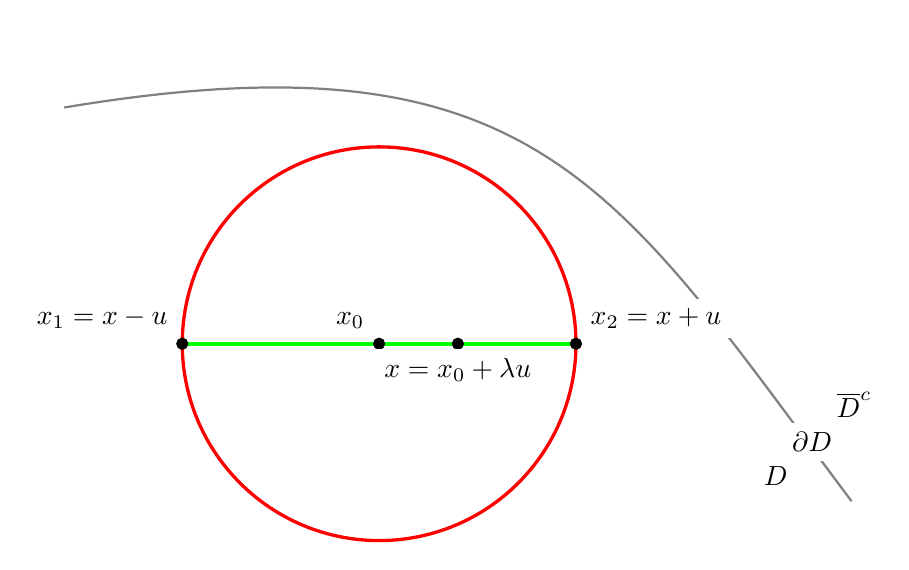
\begin{tikzpicture}
    \draw[gray, thick] (0, 5) .. controls (6, 6) and (7, 4) .. (10, 0);
    \draw[red, very thick] (4, 2) circle(2.5);
    \draw[green, ultra thick] (1.5, 2) -- (6.5, 2);
    \filldraw[black] (4, 2) circle(2pt);
    \node[above left=0pt of {(4, 2)}, outer sep=2pt, fill=white] {\( x_{0} \)};
    \filldraw[black] (5, 2) circle(2pt);
    \node[below =0pt of {(5, 2)}, outer sep=2pt, fill=white] {\(
    x=x_{0}+\lambda u \)};
    \filldraw[black] (1.5, 2) circle(2pt);
    \node[above left=0pt of {(1.5, 2)}, outer sep=2pt, fill=white] {\( x_{1}=x-u \)};
    \filldraw[black] (6.5, 2) circle(2pt);
    \node[above right=0pt of {(6.5, 2)}, outer sep=2pt, fill=white] {\(
    x_{2}=x+u \)};
    \node[above right=5pt of {(9.5, 0.75)}, outer sep=2pt, fill=white] {\( 
    \overline{D}^{c}\)};
    \node[below left=5pt of {(9.5, 0.75)}, outer sep=2pt, fill=white] {\(
    D\)};
    \node[, outer sep=2pt, fill=white] at (9.5, 0.75) {\(
    \partial D\)};
  \end{tikzpicture}

  Let \( u = x - x_{1} \), then \( x_{1} = x - u \), \( x_{2} = x+ u \) and
  there exists some \( \lambda > 0 \) such that \( x = x_{0} + \lambda u \).

  Then, we have
  \begin{align*}
    x = x_{0} + \lambda u = x_{0} + \lambda (x_{2} - x_{0}) = \lambda x_{2} + (1
    - \lambda) x_{0}\\
    \implies f(x) \le \lambda f(x_{2}) + (1- \lambda) f(x_{0})
  .\end{align*}, and
  \begin{align*}
    x &= x_{0} + \lambda u = x_{0} + \lambda ( x_{0} - x_{1}) \\
    &\implies x_{0} = \frac{1}{\lambda + 1} x + \frac{\lambda}{\lambda + 1}
    x_{1}\\
    &\implies f(x_{0}) \le  \frac{1}{\lambda + 1} f(x) + \frac{\lambda}{\lambda +
    1} f(x_{1})
  .\end{align*}

  Let \( M = \sup_{x \in \partial B(x, \varepsilon)} f(x) \) , then \( M \ge
  f(x_{1}), f(x_{2}) \) and \( f(x) \le  \lambda M + (1-\lambda)f(x_{0}) \) and
  \( f(x_{0}) \le \frac{1}{\lambda+1} f(x) + \frac{\lambda}{\lambda+1} M \).
  Another thing to note is that \( M \) is finite due to \( f \) not yielding
  any infinities.

  Hence, we have the following inequalities:

  \begin{align*}
    f(x) - f(x_{0}) &\le  \lambda(M - f(x_{0}))\\
    f(x) + \lambda M &\ge (\lambda + 1) f(x_{0})\\
    \implies f(x) - f(x_{0}) &\ge  \lambda (f(x_{0}) - M)
  .\end{align*}

  Hence, \( 0 \le  |f(x) - f(x_{0})| \le  \lambda (M-f(x_{0})) \), and let \( x \to
  x_{0} \), then \( \lambda \to  0 \) and therefore by the squeeze theorem, \(
  f(x) \to  f(x_{0}) \). Therefore \( f \) is continuous at \( x_{0} \).
\end{proof}

\begin{theorem}
  Let \( f \) be a function on open convex set \( D \).

  If \( f \) is convex, then for all directions \( d \neq  0 \),
  \( \frac{\partial f}{\partial d}(x_{0})  \), the
  \textbf{directional derivative} of \( f \) at \( x_{0} \in D \) wrt direction
  \( d \) exists and satisfies \( \frac{\partial f}{\partial d} (x_{0}) \le f(x_{0} + d) -
  f(x_{0}) \) if \( x_{0} + d \in D \).

  If \( f \) is differentiable, \( \nabla f = f'^{T} \) is the \textbf{gradient}
  of \( f \) exists. Then \( f \) is convex iff \( f(y)-f(x) \ge f'(x)(y-x)
   = \langle \nabla f(x), y -x\rangle\) for all \( x,y\in D \). Moreover, \( f
   \) is strictly convex on \( D \) iff equality only holds if \( x = y \).
\end{theorem}

\begin{proof}
  Consider the scalar function \( g(t) = f(x_{0}+t d) \), then \( g \) is
  defined on some neighborhood \( B(0, \varepsilon) \) of \( 0 \).

  We will prove that \( g \) is convex. This is true since \( g(\mathcal{C}(T,
  \lambda)) = f(x_{0} + \mathcal{C}(T, \lambda)d) = f(\mathcal{C}(x_{0} + Td,
  \lambda) \), because of linearity. Since \( f \) is convex \( g(\mathcal{C}(T,
  \lambda)) = f(\mathcal{C}(x_{0}+Td, \lambda)) \le \mathcal{C}(f(x_{0}+Td),
  \lambda) = \mathcal{C}(g(T), \lambda) \), QED.

  Then, we just need to prove that \( g \) has right derivative at \( 0 \). This
  is indeed true, as for any \( 0 < u < v < \varepsilon \), if let \( \lambda =
  \frac{u}{v}\), then \( u = \lambda v + (1 - \lambda) 0 \) and \( g(u) \le
  \lambda g(v) + (1- \lambda)g(0) = \lambda g(v) + (1 - \lambda)g(0) \). Hence,
  \( \frac{g(u) - g(0)}{u} \le  \frac{g(v) - g(0)}{v} \), and the function
  \( h(x) = \frac{g(x) - g(0)}{x} \) is decreasing as \( x \to  0^{+} \). Hence,
  there is a limit \( L = \lim_{x \to 0^{+}} h(x)  \), which is the right
  derivative of \( g(x) \) at \( 0 \). Note that this derivative can be
  (negative) infinity, for example if \( g(x) = -\sqrt[3]{x}  \).

  In the case that \( x_{0} + d \in D \), \( h(1) \) is defined as \( h(1) =
  g(x_{0}  + d) - g(x_{0}) \ge  L = \frac{\partial f}{\partial d}(x_{0})  \), QED.

  Letting \( d = y - x \), then using the identity \( \frac{\partial f}{\partial
  d} (x_{0}) = f'(x_{0})d \) for differentiable \( f \), we have \( f(y)-f(x)
  \ge f'(x)(y-x) \) for all \( x, y \in D \) if \( f \) is convex.

  To prove the reverse direction, let \( x = \mathcal{L}(y, z, w) \) such that \(
  w \in [0, 1]\) (denoting \( \mathcal{L}(x, y, w) = wx + (1-w)y \) as the
  \textbf{linear interpolation} (lerp) from \( x \) to \( y \) with weight \( w \)).
  Then, \( f(z)-f(x) \ge f'(x)(z-x) \) and \( f(y)-f(x) \ge f'(x)(y-x) \).
  Lerping the two inequality: \( \mathcal{L}(f(y)-f(x),f(z)-f(x),w) \ge
  f'(x)\mathcal{L}(y-x, z-x, w) \), yields \( \mathcal{L}(f(y), f(z), w) - f(x)
  \ge  f'(x)(\mathcal{L}(y,z,w)-x\). RHS is \( 0 \) since \( x =
  \mathcal{L}(y,z,w) \), which means \( \mathcal{L}(f(y), f(z), w) \ge
  f(\mathcal{L}(y,z,w) \), which implies that \( f \) is convex.

  To prove the theorem in the strictly convex case, we can trivially use the
  above proof with some obvious modifications.
\end{proof}

Now, consider \( f: D \subseteq \mathbb{R}^{n} \to  \mathbb{R} \), then \(
\nabla f: D \subseteq \mathbb{R}^{n} \to  \mathbb{R}^{n} \), which is a vector
function. Hence, one can define the Jacobian of this function \( (\nabla f)' \).
This matrix, if it exists, is called the \textbf{Hessian} of \( f \). And in
most cases, it's symmetric, hence it could be written as \( (\nabla f)'^{T} =
\nabla ^2 f \). Then, one have the Taylor theorem: for a
twice-continuously-differentiable function \( f \) and \( x_{0}, \Delta x \)
such that \( x_{0}, x_{0} + \Delta x \in \operatorname{dom} f \), then there
exists some \( \theta \in [0, 1] \) such that:

\begin{align*}
  f(x_{0}+\Delta x) &= f(x_{0}) + f'(x_{0})\Delta x + \frac{1}{2} \Delta x^{T}
  \nabla ^2f(x_{0} + \theta \Delta x) \Delta x\\
&= f(x_{0}) + f'(x_{0})\Delta x + \frac{1}{2} \Delta x^{T}
  \nabla ^2f(x_{0}) \Delta x + o(\|\Delta x\|^2)
.\end{align*}

Using this theorem, one can prove the following important result, which can be
used to identify convex functions.

\begin{theorem}[Second derivative test for convex functions]
  Let \( f \) be a twice-continuously-differentiable function on an open convex
  domain \( D \). Then, \( f \) is convex iff \( \nabla ^2 f(x) \) is
  positive semi-definite. Moreover, \( f \) is strictly convex if \( \nabla ^2
  f(x) \) is positive definite.
\end{theorem}

\begin{proof}
  Rewrite Taylor theorem as
  \[
    f(x_{0}+\lambda d)-f(x_{0})-\lambda f'(x_{0})d =\lambda^{2}
    \frac{d^{T}\nabla^{2}f(x_{0} + t\lambda d)d}{2}
  .\], then \( f \) is convex iff LHS is non-negative for all \( x_{0}, \lambda
  \) and \( d \). Hence, if \( \nabla ^2 f \) is positive semi-definite, then
  RHS is non-negative and we have QED.

  If \( f \) is convex, then we use the other variant of the Taylor's theorem
  and have RHS equals to \( \frac{1}{2}\lambda ^2 d^{T}\nabla ^2 f(x_{0})d +
  o(\lambda ^2) \), which is dominated by the first term. Hence, \( \nabla ^2
  f(x_{0}) \) needs to be positive semi-definite for all \( x_{0} \in D \).

  The strictly convex case could be similarly proven.
\end{proof}

After all of that theory about convex functions, we have the following theorem,
which states a valuable property about convex minimization problems.

\begin{theorem}
  Consider the minimization problem \( P: \min f(x), x \in D \), with \( D \) being
  a convex set, \( f(x) \) convex on \( D \). Then, if \( P \) has a LOS \(
  x_{0} \), then \( x_{0} \) is also a GOS. Moreover, if \( f \) is strictly
  convex, then \( x_{0} \) is the SGOS of \( P \).
\end{theorem}

\begin{proof}
  Let \( x_{0} \) be a \( B(x_{0}, \varepsilon) \)-optimal solution of \( P \).

  Then for any \( x \in D \) that is more optimal than \( x_{0} \),
  any convex combination of \( x_{0} \) and \( x \) would be more optimal than
  \( x_{0} \). We will prove that there is one such combination \( x' =
  \mathcal{L}(x_{0}, x, w) \in B(x_{0}, \varepsilon) \setminus \{x_{0}\}   \).

  We can easily prove that \( d(x_{0}, x') = \|x'-x_{0}| = w|x-x_{0}| \), which
  can be arbitrary small (but still positive)
  s.t. \( w > 0 \), which means that one can always pick
  some \( w \) such that \( x' \in B(x_{0}, \varepsilon) \) and \( x' \) is more
  optimal than \( x_{0} \). Hence, there is no \( x \in D \) that is more
  optimal than \( x_{0} \).

  If \( f \) is strictly convex, then any convex combination of \( x_{0} \) with
  an \( x \neq  x_{0}  \) that is at least as optimal as \( x_{0} \)
  would be more optimal than both \( x \) and \( x_{0} \). Hence, such \( x \)
  could not exist, and \( x_{0} \) is the SGOS of the problem.
\end{proof}

% subsection Convex optimization problem (end)

% section General optimization problem (end)

% chapter General optimization problem (end)

    \chapter{Linear programming} % (fold)
\label{sec:Linear programming}

\section{General, standard form and augmented form linear programs} % (fold)
\label{sec:General, standard form and augmented form linear programs}

The most general form of a linear program is the following optimization problem.

\begin{align*}
  \min\, &f(x) = cx\\
  \text{s.t.}\, & Ax\ge b, x \in \mathbb{R}^{n}
.\end{align*}, for matrices \( A \in \mathbb{R}^{m \times n}\), row vector
\(c \in \mathbb{R}^{ 1\times  n} \).

\( m, n \) are called as the \textbf{number of variables} and the \textbf{number
of constraints} of the problem, respectively.

e.g. $\min f(x)=5x_{1}-6x_{2}+3x_{3}$ s.t. $8x_{1}+6x_{2}+6x_{3}=5$, $3x_{1}-2x_{2}+7x_{3}\geq 7$ and $x_{1},x_{2},x_{3}\geq 0$ has

\renewcommand\arraystretch{1.3}

\[
  [A|b]=\mleft[
  \begin{array}{ccc|c}
8 & 6 & 6 & 5 \\
-8 & -6 & -6 & -5 \\
3 & -2 & 7 & 7 \\
1 &  &  & 0 \\
 & 1 &  & 0 \\
	 &  & 1 & 0 \\
   \end{array}
   \mright], c=\begin{bmatrix}
5 & -6 & 3
\end{bmatrix}
\] (omited entries are \( 0 \))

As one can see, general form linear programs can model many different types of
constraints, like regular inequalities, equalities, and non-negative
requirements.

However, we will focus on solving a restricted form of the general problem, and
provide one a method to convert from any arbitrary general problem to a
restricted problem.

\begin{definition}
  A \textbf{standard form linear program} (SFLP) is an optimization problem in the
  form:
  \begin{align*}
  \min\, &f(x) = cx\\
  \text{s.t.}\, & Ax\ge b, x \ge  0
  .\end{align*}

  An \textbf{augmented form linear program} (AFLP) is an optimization problem in the
  form:
  \begin{align*}
  \min\, &f(x) = cx\\
  \text{s.t.}\, & Ax=  b, x \ge  0
  .\end{align*}
\end{definition}

To convert from the augmented form of a linear program to the standard form, one
can use the duplication trick as the above example, or even better, introduce a
new variable for each constraint. Such variables are called \textbf{slack
variables}.

\begin{align*}
  z &= \begin{bmatrix} x \\ y \end{bmatrix} \in \mathbb{R}^{n + m}\\
  A' &= \begin{bmatrix} A & I_{m} \end{bmatrix} \in \mathbb{R}^{m \times (n +
  m)}\\
    Ax \ge b &\iff y = b - Ax \ge  0\\
     &\iff  z \ge 0 \text{ and } Az = b
.\end{align*}, and
\begin{align*}
  &c' = \begin{bmatrix} c & 0_{m} \end{bmatrix} \in \mathbb{R}^{n + m}\\
  \implies f(x) &= cx = c'z = g(z)
.\end{align*}

Hence, the SFLP is equivalent to the following AFLP

  \begin{align*}
  \min\, &g(z) = c'z\\
  \text{s.t.}\, & A'z=  b, z \ge  0
  .\end{align*}

Converting from a general linear program to an SFLP is not as straightforward.
For every unbounded variables \( x^{i} \), let \( x^{i} = y^{i} - z^{i} \) for
some non-negative \( y^{i}, z^{i} \)
Then, the general problem is equivalent to the following SFLP

\begin{align*}
  \min\,&g(x') = c'x'\\
  \text{s.t.}\,& A'x' \ge  b, x' \ge  0
.\end{align*}, with 
\begin{align*}
  x' &= \begin{bmatrix} y \\ z \end{bmatrix} \in \mathbb{R}^{2n}\\
  A' & = \begin{bmatrix} A & -A \end{bmatrix} \in \mathbb{R}^{m \times  2n}\\
  c' &= \begin{bmatrix} c & -c \end{bmatrix} \in \mathbb{R}^{1 \times  2n} 
.\end{align*}.

Of course, this is the general case. In practice, one would want to minimize the
number of constraints and variables to make thing much easier to handle, by
utilizing "prebounded" and "already-slack" variables in the problem.
% section General, standard form and augmented form linear programs (end)

\section{Convex polyhedra} % (fold)
\label{sec:Convex polyhedra}

\subsection{Hyperplanes and related theorems} % (fold)
\label{sub:Hyperplanes and related theorems}

Consider the feasible for the above problem: \( D = \{x, Ax\ge b\}   \). Then,
one can see that \( D \) is the intersection of sets \( H_{i}=\{x, A^{i}x \ge
b^{i}\}   \) for \( i \) ranging from \( 1 \) to \( m \).

Now, we will have some names for these sets.

\begin{definition}
  A \textbf{hyperplane} is a set \( H \) in the form of \( H = \{x, ax =
  \alpha\}   \). \( H \) splits the whole space into two open sets, which are
  called \textbf{open half-spaces}: \( H_{1} = \{x, ax > b\}   \) and \( H_{2}
  = {x, ax < b} \). There are also closed half spaces \( H_{3} = H_{1} \cup H =
  \{x, ax \ge  b\}  \) and \( H_{4} = H_{2} \cup  H = \{x, ax \le  b\}   \). The
  vector \( a^{T} \) is the \textbf{normal} of \( H \).

  Let \( S \subseteq \mathbb{R}^{n} \) and \( x_{0} \in S \). Then, a hyperplane
  \( H = \{x, ax = \alpha\}   \) is a \textbf{supporting hyperplane} of \( S \)
  at \( x_{0} \) iff \( x_{0} \in H \) and either \( S \subseteq H_{1} \) or \(
  S \subseteq H_{2}\), with \( H_{1}, H_{2} \) being the closed half-spaces
  bounded by \( H \).

  Let \( A, B \) be two subsets of \( \mathbb{R}^{n} \). Then, a hyperplane \( H
  \) \textbf{separates} \( A \) and \( B \) if and only if \( H \) splits the \(
  \mathbb{R}^{n}\) space into two closed half-spaces \( H_{1} \) and \( H_{2} \)
  such that \( A \subseteq H_{1} \) and \( B \subseteq H_{2} \).
\end{definition}

Before going on proving the important hyperplane theorems, we start with a
simple lemma.

\begin{theorem}
  Let \( S \) be a nonempty closed set in \( \mathbb{R}^{n} \). Then for every
  \( x_{0} \in S^{c} \), there exists some \( x_{1} \in S \) such that \(
  d(x_{0}, x_{1}) \le d(x_{0}, x), \forall x \in S \).
\end{theorem}

\begin{proof}
  Note that this is basically a minimization problem: \( \min f(x) = d(x_{0}, x), x \in
  S\), then we can use the theorems in the last chapter to prove that a GOS
  exist. We will use Theorem \ref{thr:coercive condition}, which requires \(
  f(x) \) to be (lower semi-)continuous and \( \lim_{x \to \infty} f(x) = +\infty \), which are both trivial to prove.
\end{proof}

\begin{theorem}[Hyperplane Separation Theorem (Closed set-point variant)]
\label{thr:hst-closed-pt}
  Let \( S \) be a nonempty, convex, closed set. Then for every \( x_{0} \in S^{c}
  \), there exists some hyperplane separating \( S \) and \( \{x_{0}\}   \).
\end{theorem}

\begin{proof}
  Let \( x_{1} \) be the closest point on \( S \) to \( x_{0} \), denote \( d =
  (x_{1}-x_{0})^{T}\).

  Then, we will prove that the hyperplane \( H = \{x, dx = dx_{1}\}   \) is a
  supporting hyperplane of \( S \). If this is true, then it's trivial that \( H
  \) separates \( S \) and \( \{x_{0}\}   \).

  Now, we have \( dx_{0}-dx_{1}=-d^{T}d < 0 \), which means that \( x_{1} \in
  H_{1} = \{dx < dx_{1}\}   \). Hence, we need to prove that \( S \subseteq
  H_{2} = \{dx \ge  dx_{1}\}   \), or \( x \in S \implies dx \ge  dx_{1} \).

  Assuming that there is some \( x_{2} \in S \) such that \( dx_{2} < dx_{1} \).
  Consider the lerp between \( x_{2} \) and \( x_{1} \): \( x(\lambda) =
  \operatorname{lerp}(x_{2}, x_{1}, \lambda) \), which must be in \( S \) for
  every \( \lambda \in [0, 1] \)
  \begin{align*}
    x(\lambda) - x_{0} &= \operatorname{lerp}(x_{2}, x_{1}, \lambda) -
    x_{0}\\
                       &= \operatorname{lerp}(x_{2}-x_{1}, 0, \lambda) + (x_{1}
                       - x_{0})\\
                       &= \lambda(x_{2}-x_{1}) + d^{T}\\
  .\end{align*}

  \begin{align*}
    \|x(\lambda)-x_{0}\|^2 &= (\lambda(x_{2}-x_{1}) + d^{T})^{T}(\lambda(x_{2}-x_{1})
    + d^{T})\\
                           &= \|d\|^2 + 2\lambda d(x_{2}-x_{1}) + \lambda
                           ^2\|x_{2}-x_{1}\|^2\\
                           &= \|x_{1}-x_{0}\|^2 + \lambda g(\lambda)
  .\end{align*},
  with \( g(\lambda) = 2d(x_{2}-x_{1}) + \lambda \|x_{2}-x_{1}\|^2 < 0 \) for
  small \( \lambda > 0 \), which means that \( \lambda g(\lambda) < 0 \) and
  therefore \( x(\lambda) \) is closer to \( x_{0} \) than \( x_{1} \), which is
  a contradiction.
\end{proof}

\textbf{Remark. } The hyperplane constructed above is a supporting hyperplane of
\( S \) at \( x_{1} \).

\begin{corollary}
  A closed convex set \( S \) is the intersection of the closed half-spaces that
  contains \( S \).
\end{corollary}

\begin{proof}
  If \( x \in S \), then every closed half-space that contains \( S \) contains
  \( x \).

  If \( x \in S^{c} \), then there exists a supporting hyperplane separating \(
  S\) and \( \{x\}   \), which means that \( x \) could not be in the close
  half-space that \( S \) is in.
\end{proof}


\begin{theorem}[Supporting Hyperplane Theorem]
  \label{thr:sht-boundary}
  Let \( S \) be a nonempty convex set and a point \( x_{0} \in \partial S \).
  Then, there exists a supporting hyperplane of \( S \) at \( x_{0} \).
\end{theorem}

\begin{proof}
  In every open ball \( B(x_{0}, \varepsilon_{n}) \), pick a point \( x_{n} \in
  B(x_{0}, \varepsilon_{n}) \cap  S^{c}\). Then, \( \lim_{n \to \infty} x_{n} =
  x_{0}\) if \( \varepsilon_{n} \to  0 \), which we will fix to \( \varepsilon_{n}
  = \frac{1}{n}\) for example.

  Using the previous theorem, there exists hyperplanes \( H_{n} \) separating \(
  S\) from \( \{x_{n}\}   \). Let the normal unit vector of \( H_{n} \) be \(
  d_{n} \), with the convention that \( d_{n}(x-x_{n}) \ge 0, \forall  x \in
  S \).

  Hence, \( d_{n} \) is a sequence on the compact set \( \partial B(0, 1) \),
  which means that there must be a convergent subsequence \( d_{i_{n}} \) that
  converges to \( d \).

  Since \( d_{n}(x-x_{n}) \ge 0 \) for all \( x \in S \), letting \( n = i_{m}
  \) and \( m \to  \infty \), we have \( d(x-x_{0}) \ge 0 \), and therefore \(
  H=\{x, d(x-x_{0})\ge 0\}   \) is a supporting hyperplane of \( S \).
\end{proof}

\begin{corollary}[Hyperplane Separation Theorem (Set-point variant)]
\label{cor:hst-set-pt}
  Let \( S \) be a nonempty convex set, then for every \( x \in
  (\operatorname{Int} S)^{c} \), there is a supporting hyperplane \( H \) that
  separates \( S \) and \( \{ x\}   \).
\end{corollary}

\begin{proof}
  If \( x \in \partial S \), the supporting hyperplane exists due to Theorem
  \ref{thr:sht-boundary}.

  If \( x \in \overline{S}^{c} \), then if \(\overline{S} \) is a convex set,
  there exists a supporting hyperplane of \( \overline{S} \) at \( x \), which
  is also a supporting hyperplane of \( S \) at \( x \), due to Theorem
  \ref{thr:hst-closed-pt}.

  To conclude, one would need to prove that \( \overline{S} \) is convex, using
  the following lemma.
  \begin{lemma}
    Let \( S \) be a convex set. Then \( \overline{S} \) is also a convex set.
  \end{lemma}

  \begin{proof}[Proof of lemma]
    Consider \( x \in \overline{S} \). If \( x \in S \), then there is a trivial
    sequence \( x_{n} = x \) that converges to \( x \). Otherwise, if \( x \in
    \partial S \), then every neighborhood \( B(x, \varepsilon_{n}) \) of \( x
    \) has at least some point in \( S \), which will be denoted as \( x_{n} \).
    Then, the sequence \( x_{n} \) converges to \( x \) if one let \(
    \varepsilon_{n} \to  0 \) as \( n \to  \infty \), for example \(
    \varepsilon_{n} = \frac{1}{n} \). Hence, for every \( x \in \overline{S} \),
    there is always a sequence \( x_{n} \in S \) that converges to \( x \).

    Consider a subset \( A \subseteq \overline{S} \), then there exists a
    sequence of sets \( A_{n} \) that converges to \( A \).

    Then, \( x_{n} = \mathcal{C}(A_{n}, \lambda) \to  \mathcal{C}(A, \lambda) =
    x\) because of linearity, as \( n \to  \infty \). Note that \( x_{n} \in S
    \) and we need to prove that \( x \in \overline{S} \), which is the reverse
    direction of what we've just proven above.

    If \( x \notin \overline{S} \), then there exists a neighborhood \( B(x,
    \varepsilon) \) of \( x \) that does not intersect \( \overline{S} \).
    However, that neighborhood must contain infinitely many points in the
    sequence \( x_{n} \), which is a contradiction.

    Hence, \( x \in \overline{S} \), and therefore \( \overline{S} \) closed
    under convex combination.
  \end{proof}
\end{proof}

Finally, we can prove the \textbf{Hyperplane separation theorem}.
\begin{theorem}[Hyperplane Separation Theorem]
  Let \( A, B \) be nonempty disjoint convex sets, then there exists a
  hyperplane that separates the sets.
\end{theorem}

\begin{proof}
  Consider the set \( S = S_{1} - S_{2} = \{s_{1} - s_{2},
  s_{1} \in S_{1}, s_{2} \in S_{2}\}   \).

  \( S \) is convex, since if \( x_{1}-x_{2}, y_{1}-y_{2} \in S_{1}-S_{2} \)
  (s.t. \( x_{1},y_{1} \in S_{1}, x_{2}, y_{2} \in S_{2} \)), then a convex
  combination of the two, which can be written as \(
  \operatorname{lerp}(x_{1}-x_{2},y_{1}-y_{2},\lambda) =
  \operatorname{lerp}(x_{1},y_{1},\lambda) -
  \operatorname{lerp}(x_{2},y_{2},\lambda) \in S_{1}-S_{2} \) due to the fact
  that \( operatorname{lerp}(x_{i},y_{i}, \lambda) \in S_{i} \).

  Then, using Corollary \ref{cor:hst-set-pt}, there is a hyperplane separating
  \( S_{1}-S_{2} \) and \( \{0\}   \). Moreover, there is one such hyperplane
  that passes through \( 0 \), which could be constructed by slightly modifying
  the proofs of the above theorems. Denote this hyperplane as \( H = \{x, dx \ge
  0\}   \), then we have \( dx_{1} \ge  dx_{2}, \forall x_{1} \in S_{1}, x_{2}
  \in S_{2} \).

  Let \( \alpha = \inf dS_{1}, \beta = \sup dS_{2} \), then we have \( dx_{1}
  \ge  \alpha \ge  \beta \ge dx_{2}, \forall x_{1} \in S_{1},x_{2} \in S_{2} \),
  which yields at least one separating hyperplane of \( S_{1} \) and \( S_{2}
  \): \( H'(\gamma) = \{ dx = \gamma\}   \) for any \( \gamma \in [\alpha,\beta]
  \), which is a nonempty interval.
\end{proof}

% subsection Hyperplanes and related theorems (end)

\subsection{Extreme points and recession directions} % (fold)
\label{sub:Extreme points and recession directions}

\begin{definition}
  Let \( S \) be a subset of \( \mathbb{R}^{n} \).

  If \( S \) is convex, then \( x \in S \) is an \textbf{extreme point} if and only if
  it could not be written as a strictly convex combination of a collection
  of points in
  \( S \) not containing \( x \). In other words, \( x \in S \) is an extreme
  point if for every \( y, z \in S \setminus \{x\}, w \in (0, 1)   \), we have
  \( x \neq \operatorname{lerp}(y,z,w) \).

  If a vector \( v \) satisfies, \( x + tv \in S \) for every \( x \in S \), \(
  t \ge  0\), then \( v \) is a \textbf{recession direction} of \( S \).

  A recession direction \( v \) is called a \textbf{extreme direction} if it is
  not a strictly convex combination of any collection of recession directions
  not containing directions in the form \( kv \) for scalars \( k \in \mathbb{R}
  \).
\end{definition}

Now, we will prove a very important result of extreme points and its compact
convex set: the \textbf{Krein-Milman Theorem}. But before proving the whole
theorem, we will look at a lemma about \textbf{faces}.

\begin{lemma}
  Let \( S \) be convex compact set on \( \mathbb{R}^{n} \). Then a \textbf{face}
  \( F \)
  of \( S \) is a subset \( F \subseteq S \) such that if \( z =
  \operatorname{lerp}(x, y, w) \in F \) for some \( x, y \in S, 0 < w < 1 \),
  then \( x, y \in F\).

  Let \( c \) be a row vector, then the set \( F_{c}(S) = \operatorname{Argmax}
  \{cx, x \in S\}     \) is a face.

  An extreme point of a face \( F \) of \( S \) is also an extreme point of \( S
  \).
\end{lemma}

\begin{proof}
  If \( x = \operatorname{lerp}(y,z, w) \in F_{c} \) for some \( y,z \in S \),
  then \( cx = \operatorname{lerp}(cy, cz, w) \le \max \{cy, cz\}   \), which
  means that either \( y \) or \( z \) is a GOS of the problem. WLOG assuming \(
  cx = cy\), then we end up having \( cz = cx \). Therefore, \( y, z \in F_{c}
  \), and \( F_{c} \) is a face of \( S \).

  To prove the second statement, let \( x \) be an extreme point of \( F \).
  Assuming that there exists \( y, z \in S, \lambda \in (0, 1) \) such that \( x =
  \operatorname{lerp}(y, z, \lambda) \), then \( y, z \in F \) because of the
  definition of faces, which leads to a contradiction.
\end{proof}

\begin{theorem}[Krein-Milman Theorem (Existence)]
  Let \( S \) be a nonempty, compact and convex set. Then, \( S \) has at least
  one extreme point.
\end{theorem}

\begin{proof}
Denote \( S_{1} = S \). Then for every \( i \), assuming \( S_{i} \) is a
nonempty face (induction hypothesis). There will be some cases
\begin{itemize}
  \item If \( |S_{i}| = 1 \) and \( S_{i} = \{ s\}   \), then \( s \) is an
    extreme point of \( S \).
  \item If \( |S_{i}| \ge  2 \), then pick \( x, y \in S_{i}, x \neq y \). Then,
    consider the hyperplane \( H: ax = \alpha \) separating \( x \) and \( y \),
    i.e. \( ax < \alpha < ay \), which always exist. Then, let \( S_{i+1}
    \coloneqq F_{a}(S_{i}) \subset S_{i} \), which is a nonempty face that is a
    proper subset of \( S_{i} \) (since \( x \notin F_{a} \)).
\end{itemize}

Consider the family \( \mathcal{A} \) of all nonempty faces of \( S \), with the partial
order \( \subseteq \). Then, the above procedure will have to halt at some
point (Zorn's lemma).
\end{proof}

\begin{theorem}[Krein-Milman Theorem]
  Let \( S \) be a nonempty, compact and convex set. Then, \( S \) is the convex
  hull of \( E(S) \), the set of its extreme points.
\end{theorem}

\begin{proof}
  Using the previous theorem, one can see that \( E(S) \) is nonempty.
  Let \( T \) be the convex hull of \( E(S) \), then one can trivially
  see that \( T \subseteq S \). Assuming there exists \( x \in T \setminus S \),
  then by the Hyperplane Separation Theorem, there is a row vector \( a \) such
  that \( \sup aT < ax \).

  Consider the face \( F_{a} = \operatorname{Argmax} \{ ax, x \in S \}   \),
  then \( T \cap  F_{a} = \varnothing \). Then, the face \( F_{a} \) would have
  an extreme point \( e' \), which means that \( e'  \notin E(S)\), which is a
  contradiction.
\end{proof}

% subsection Extreme points and recession directions (end)

\subsection{Convex polyhedra} % (fold)
\label{sub:Convex polyhedra}

\begin{definition}
  A \textbf{convex polyhedron} (plural \textit{convex polyhedra}) \( P \) is
  the intersection of finitely many closed half-spaces.

  A \textbf{convex polytope} is a bounded convex polyhedron.
\end{definition}

Then, one can write \( P \) as \( P = \{x, Ax \ge  b\}   \) for some matrix \( A
\) and row vector \( b \), with the closed half-spaces defining \( P \) being
the half-spaces \( H_{i}: A^{i}x \ge  b^{i} \).

Now, we will prove the following theorem.

\begin{theorem}[Minkowski's Theorem for Polyhedra]
  Denote \( \operatorname{conv} V \) as the convex hull of \( V \) and \(
  \operatorname{cone} R \) as the conic hull of \( R \).

  Let \( P \) be a convex polyhedron, then \( P \subseteq \operatorname{conv} E(P) +
  \operatorname{cone} R(P)\), with \( E(P), R(P) \) denoting the set of all
  extreme points and extreme directions of \( P \), respectively.
\end{theorem}

\begin{proof}

\( P \subseteq \operatorname{conv} E(P) + \operatorname{cone} R(P) \) is equivalent to
the fact that \( \forall x\in P, x = e_{i}\lambda^{i} + r _{j}\mu ^{j} =
e\lambda + r\mu \), with \( e \) and \( r \) being matrices with columns being
extreme points and extreme directions of \( P \), respectively. The condition
for the vectors \( \mu  \) and \( \lambda \) are \( \mu  \ge 0 \) and \(
\sum_{i} \lambda_{i} = 1 \)

Now, let
\begin{align*}
  x' &= \begin{bmatrix} x \\ 1 \end{bmatrix} \\
  A' &= \begin{bmatrix} A & -b \end{bmatrix} 
.\end{align*},
then \( Ax \ge b \) only if \( A'x' \ge  0 \).

Consider the convex cone \( C = \{x', A'x' \ge  0\}   \). If one can
prove the theorem for \( C \), which has no non-zero extreme points, then \(
\forall x' \in C, x' = r'\mu' \).

Observes that there are two types of extreme direction in \( D \), one with the
\( (n+1) \)-th component being \( 0 \) and one with that component being a
positive value, which could be normalized to \( 1 \) without loss of generality. Then, split \( r' \) according to this categorization, \( v \) is the matrix
that contains all extreme directions of the first type and \( u \) containing
extreme directions of the second type.

Then, there exists \( \lambda, \nu \ge 0 \) such that \( x' = u\lambda + v\nu \).
Moreover, \( 1 = x'^{n+1} = u^{n+1}\lambda= \sum_{i} \lambda^{i} \) since \(
u^{n+1}_{i} = 1 \) for all \( i \), since the extreme directions of the second
type is already normalized (wrt its last component).

Now, denote \( U = u^{1..n}, V = v^{1..n} \), we have \( x = x'^{1..n} =
U\lambda+V\nu \). This suggests that \( U \) and \( V \)'s columns are
extreme points and extreme directions of \( P\), respectively. This can be
trivially proven as follows
\begin{align*}
  0 \le  A'u_{i} = \begin{bmatrix} A & -b \end{bmatrix}  \begin{bmatrix} U_{i}
\\ 1 \end{bmatrix}  = AU - b
.\end{align*}
Hence, \( U \in P \). If \( U \) is a strict convex combination of two other \(
X_{1}, X_{2} \in P\), then \( u \) is a strict convex combination (wrt the same
weight) of the two extreme directions of \( C \) \( x_{1}, x_{2} \) given by:
\begin{align*}
  x_{i} = \begin{bmatrix} X_{i} \\ 1 \end{bmatrix}, i \in \{1, 2\}  
.\end{align*}, which is a contradiction to the fact that \( u \) is an extreme
direction of \( C \).
\begin{align*}
  0 \le  A'v_{i} = \begin{bmatrix} A & -b \end{bmatrix} \begin{bmatrix} V_{i} 0
\end{bmatrix}  = AV_{i}
.\end{align*}

Hence, \( V_{i} \) is a recession direction of \( P \) due to the fact that \(
\forall x \in P, t \ge  0, A(x+tV_{i}) = Ax + tAV_{i} = Ax \ge  b \). Using the
same logic as above, we can prove that \( V_{i} \) is an extreme direction of \(
P\).

\end{proof}

Therefore, the proof would be completed if we have proven the theorem for the
convex cone case:

\begin{theorem}[Minkowski's Theorem for Cones]
  Let \( C = \{x, Ax \ge  0\}   \) be a polyhedral cone, then \( C \) is
  contained in the conic hull of \( R(C) \), the set of its extreme directions.
\end{theorem}

\begin{proof}
  First, we prove that the set \( C_{1} = \{ x, \exists \lambda \ge 0, x =
  R\lambda\}   \) is a polyhedral cone, since one can use the
  \textbf{Fourier-Motzkin elimination algorithm} to turn from \( x = R\lambda,
  \lambda \ge 0 \) to \( Ax \le  0 \), which is the inequality for a polyhedral
  cone.

  Then, we say that \( (A, R) \) is a \textit{double description pair} (DDP) if
  \( Ax \le  0 \iff \exists \lambda \ge 0, x = R\lambda  \). Then, we will
  proceed to prove that \( (R^{T}, A^{T}) \) is also a DDP.

  \begin{align*}
    &R^{T}y \le 0\\
    &\iff \lambda^{T} R^{T} y \ge 0, \forall  \lambda \ge 0\\
    &\iff (R\lambda)^{T} y \ge 0, \forall  \lambda \ge 0\\
  .\end{align*}

  Let \( x = R\lambda \), then \( R^{T}y \le 0 \) iff \( x^{T}y \ge 0, \forall
  \lambda \ge 0, x = R\lambda \), or equivalently \( Ax \le  0 \). Then, the
  last statement is equivalent to \( Ax \le  0 \implies x^{T}y \le  0 \)

  To conclude this proof, we need to use \textbf{Farkas' Lemma}.

  \begin{lemma}[Farkas' Lemma]
  \label{farkas}
    \( ax \ge  0, \forall  x \) s.t. \( Ax \ge  0 \) iff \( a = yA \) for some
    row vector \( y \ge  0 \)
  \end{lemma}

  \begin{proof}[Proof of Farkas' lemma]
    If \( a = yA \), then \( ax = yAx \ge  0, \forall  Ax \ge 0 \).

    If \( ax \ge  0, \forall Ax \ge 0 \) and \( a \neq  yA, \forall  y\ge 0 \),
    then consider the set \( S = \{yA, y \ge 0\}   \). Since \( a \notin S \)
    and \( S \) is closed, using Theorem \ref{thr:hst-closed-pt}, there is a
    hyperplane \( H \) strictly separating \( S^{T} \) and \( \{ a^{T}\}   \).
    Assuming \( H = \{t, x^{T}t \ge  \alpha\}   \) satisfies \( ax  <  \alpha
    \le   \inf Sx \). Note that \( 0 \in Sx \), then \( \alpha \) must be
    non-positive. If \( \alpha < 0 \) and the hyperplane \( H' = \{ t, x^{T}t =
    0\}   \) could not separate the two sets, then there exists some \( t \in S
    \) such that \( tx < 0 \). Then, there exists \( k > 0 \) such that \( t(kx)
    < \alpha\), with \( kx \in S \), which means the original hyperplane also could
    not separate the two sets, which is a contradiction. Hence, the hyperplane
    \( H' \) could separate the two set, i.e. \( ax < 0 \le \inf Sx \). Then,
    we have \( A_{i}x \ge  0 \) for all \( i \), since \( A_{i} =
    A\mathbf{e_{i}} \in S \), with \( \mathbf{e_{i}} \) denoting the \( i \)-th
    standard basis vector, and hence \( Ax \ge 0 \). To conclude, \( ax < 0 \)
    for some \( x \) s.t. \( Ax \ge 0 \), which is another contradiction.
  \end{proof}

Continuing with the proof, we have
\begin{align*}
  &(Ax \le 0 \implies x^{T}y \le 0)\\
  &\iff(Az \ge  0 \implies z^{T}y \ge  0) \text{ (letting \( z = -x \))}\\
  &\iff \exists \lambda \ge 0,  y = \lambda A\\
  &\iff \exists  \lambda' = \lambda^{T} \ge 0, y^{T} = A^{T}\lambda'
.\end{align*}

Hence \( (R^{T}, A^{T}) \) is a DDP.

So to find \( R \), one find do Fourier-Motzkin on \( A^{T} \) to get \( R^{T}
\). Now that \( R \) exists, we have \( C = \{x, Ax \ge 0\} = \{x, \exists
\lambda \ge 0, x = -R\lambda\}  \)

Now, we will prove that \( -R_{i} \) are recession directions of \( C \).
Since \( R_{i} = R\mathbf{e_{i}}, \mathbf{e_{i}} \ge 0 \), \( R_{i} \in P \),
and \( AR_{i} \ge  0 \). Then, for every \( x \in P, t \ge 0 \), we have \( A(x
- tR_{i}) = Ax - tAR_{i} \le  0 \), which means that \( R_{i} \) is a recession
direction of \( C \). Pick columns from \( R \) to form a conical basis of \( R \)'s
column space, then this basis is able to span the recession cone of \( C \), due
to every recession direction \( d \) of \( C \) can be written as \( d =
R\lambda = R'\lambda' \) with some \( \lambda, \lambda' \ge  0 \).
\end{proof}

% subsection Convex polyhedra (end)

% section Convex polyhedra (end)

\section{Existence and properties of solutions of linear programs} % (fold)
\label{sec:Existence and properties of solutions of linear programs}

Firstly, since \( D = \{x\ge 0, Ax \ge  b\}   \) is a convex set (this can be
trivially seen due to the linearity of the convex combination operation) and \(
f(x)=cx\) is a convex (and a concave) function on \( \mathbb{R}^{n} \), then
every (S)LOS of the linear program is a (S)GOS.

The set \( D \) is already closed (why?) and \( f(x) \) is continuous, and hence
the problem will have a GOS if \( D \) is bounded.
% section Existence and properties of solutions of linear programs (end)

% chapter Linear programming (end)


\end{document}
